\documentclass[10pt,letterpaper]{article}
\usepackage{geometry}
\geometry{letterpaper, portrait, margin=0.5in}
\usepackage[utf8]{inputenc}
\usepackage{amsmath}
\usepackage{amsfonts}
\usepackage{amssymb}
\usepackage{graphicx}
\usepackage{subcaption}
\usepackage{array}
\usepackage{hyperref}
\setlength{\parindent}{0pt}
\renewcommand\refname{Related documents/articles to read:}

\begin{document}

\begin{center}
KMOS Work Documentation\\
By: Robert Burnet
\end{center}

\newpage

\tableofcontents

\newpage

\section{Introduction and Related Documents/Articles}

This is a document describing what I did over the term. Similar to a journal except more formal. The first section (May 1 - 12, 2016) details how I got started and could be used as a starting point for anyone else who will carry on the work. In short, read through the science proposal and KMOS instrument explanation, read and follow the KMOS esoreflex tutorial, then read the KMOS pipeline manual and cookbook and everything about KMOS to get familiar with it, download the data and associated calibration frames and start reducing data with esoreflex and writing scripts for working with the data. All my work and scripts can be found on my github page: github.com/rcburnet/S16work .
\begin{thebibliography}{1}
\bibitem{github}My github page for all my scripts: \url{github.com/rcburnet/S16work}
\bibitem{Proposal}Science Proposal: In $\sim$/S16work/ called proposal.pdf\\
\bibitem{KMOS instrument explanation}KMOS instrument explanation (overview, description, etc.): \url{https://www.eso.org/sci/facilities/paranal/instruments/kmos.html}\\
\bibitem{esoreflex installation}esoreflex installation (uses KEPLER to visually portray esorex pipeline workflows. Used to reduce KMOS data.): \url{http://www.eso.org/sci/software/pipelines/reflex_workflows/}\\
\bibitem{KMOS esoreflex tutorial}KMOS esoreflex tutorial: \url{ftp://ftp.eso.org/pub/dfs/pipelines/kmos/kmos-reflex-tutorial-1.6.pdf}\\
\bibitem{KMOS pipeline manual}KMOS pipeline manual: \url{ftp://ftp.eso.org/pub/dfs/pipelines/kmos/kmos-pipeline-manual-2.18.pdf}\\
\bibitem{KMOS pipeline cookbook}KMOS pipeline cookbook: \url{ftp://ftp.eso.org/pub/dfs/pipelines/kmos/kmos-pipeline-cookbook-1.5.pdf}\\
\bibitem{ESO Archive Query Form}ESO Archive Query Form: \url{http://archive.eso.org/eso/eso_archive_main.html}
\bibitem{SAMI instrument front-page}SAMI instrument front-page: \url{http://sami-survey.org/}\\
\bibitem{SAMI Early Data Release}SAMI Early Data Release (this is the data used): \url{http://sami-survey.org/edr}\\
\bibitem{ALFALFA survey data}ALFALFA survey data: \url{http://egg.astro.cornell.edu/alfalfa/data/}\\
\bibitem{K98}K98 (SFR from Halpha relation) article: \url{http://www.annualreviews.org/doi/pdf/10.1146/annurev.astro.36.1.189}\\

\end{thebibliography}
I began working on the desktop computer provided to me (stavrogin.uwaterloo.ca) but moved to my own laptop with Fedora 23 installed at a later date (May 24). Directory designations and filenames will change between the two workstations. The scripts that were developed and used on my laptop may not work on the desktop without changing directory designations in the scripts. Some of the scripts use data that are not generated for the pipeline. For instance, I had to combine observation blocks OB1 and OB2 to get the full exposure of the data, the pipeline did not combine them, and some of my scripts use the combined OB data. You will have to do that manually yourself. Document \cite{KMOS pipeline manual} and \cite{KMOS pipeline cookbook} are helpful in this regard, especially the sections on the ``kmos$\_$combine" recipe.\\

\newpage

\section{Sources' Description}
There are two clusters that we obtained KMOS data for, and for each of those clusters there are $\sim$20 targets/sources in those clusters that KMOS specifically collected data on. A description in the form of a table for the clusters and their corresponding targets/sources is shown below.\\

do table.\\

\section{Desktop work}
From May 1 - May 24 I worked on the desktop provided to me by Michael Balogh (stavrogin.uwaterloo.ca). From here on, the $\sim$ directory will refer to the /home/rcburnet/work/project$\_$data/scripts/ directory on the desktop.
\subsection{May 1: Getting Started}
Spent most of my time understanding the KMOS data, esoreflex/esorex (the software package used to reduce and calibrate the KMOS data) pipelines and recipes, especially esoreflex and how to use it to reduce KMOS data. I would start first by reading through the science proposal \cite{Proposal}, then the KMOS instrument explanation \cite{KMOS instrument explanation} and then reading and following the KMOS esoreflex tutorial \cite{KMOS esoreflex tutorial} to get an understanding of the instrument, get a feel of the data reduction process and pipelines, and getting familiar with esoreflex before anything. For information on the pipelines and recipes used to reduce KMOS data with esoreflex/esorex and to understand what esoreflex does to reduce and calibrate the data, look into documents \cite{KMOS pipeline manual} and \cite{KMOS pipeline cookbook}. I would recommend reading anything related to KMOS (documents/articles above as well as anything in the bookmarks.html bookmark file in $\sim$/S16work/bookmarks.html) after you familiarized yourself with the tutorial. The tutorial tells you how to install esoreflex and how to use it. During the installation of esoreflex, it provides you the option to download demo data you can use as you follow the tutorial. I suggest doing that to get familiar with the kinds of data you will be working with and the data reduction pipelines and recipes before going into the real data reduction yourself and reading deeper into the esoreflex/esorex pipelines and recipes as they can be a cumbersome read.\\

After going through the tutorial and reading through anything to do with KMOS and esoreflex - after getting familiar with the data and data reduction process - you should download the KMOS data that you will be working with. To download the KMOS data, use the ESO Archive Query Form \cite{ESO Archive Query Form} with program ID: 093.A-0625 . This is the program that Balogh's data was assigned with, all the data I worked with was designated by that program ID. Put that program ID under the program ID text box then click ``search" and it'll send you to the data retrieval page. Mark everything for installation, click ``request marked dataset" and sign in or sign up to the ESO User Portal. Give a good description for the data, select ``Selected files + associated raw calibrations (if available)" to select both the raw science frames and the calibration frames associated with them (to be used with the esoreflex/esorex pipelines to reduce the data and carry out calibrations), click ``submit" and then download the files to your working directory. Note that all the science frames and associated calibration frames are together over 10GB, so make sure you have the space to accommodate. Uncompress the data and you're done! Note that you will need to change your RAW$\_$DATA$\_$DIR designation in the KMOS esoreflex workflow to the directory you downloaded your raw data to so that it can use the data. Once it's all set-up, you are ready to reduce the KMOS data yourself. Read the KMOS esoreflex tutorial, pipeline manual, and cookbook if you haven't already before you run esoreflex to reduce the data so you understand what each step of the workflow does: how the calibration data is processed and used, how the science frames are reduced, etc. 

\subsection{May 12: Plotting spectrum of reduced data cubes and searching for signs of H$\alpha$}
After I familiarized myself with KMOS (the data, data reduction process, and esoreflex and its pipelines/recipes), I came across my first problem with the final reduced data cubes that esoreflex outputted after reducing the KMOS data: there was no sign of any sort of target anywhere! When looking through the data cubes is ds9, no target seemed to pop up. With the demo data, you could clearly see some bright object in the center of each cube as you go through the wavelength slices, but the KMOS data cubes had no such thing. I thought that this might be because the objects we are looking at are much fainter than the demo objects, so they won't pop out as much when going through the slices, but they should sitll have detectable and noticeable H$\alpha$ flux. Our next step was to see if we could detect any H$\alpha$.\\

I created the script ``total$\_$flux$\_$vs$\_$wavelength.py" (see $\sim$/S16work/total$\_$flux$\_$vs$\_$wavelength$\_$scripts/) to plot the spectrum of the reduced data cubes (Flux vs. Wavelength) for observation block 1 data cubes. Total flux is defined as the total sum of every pixel flux for a particular wavelength slice. I plotted that total flux against wavelength slice to see the spectrum for each target data cube in the YJ-band, as the YJ data cubes would be where H$\alpha$ would be detected. I also plotted the location of where we'd expect to see H$\alpha$ based on the red shift of the cluster that the target belonged to (either CL0034 or CL0036, see proposal for details. Note that I could have done it using each targets' individual redshift as I have the information for each target as reported in Sean's txt table files found in $\sim$/S16work/txt$\_$tables/, however at the time I didn't, I only had the redshifts for the clusters and not for each individual target which is why I plotted the location of the H$\alpha$ line for the cluster instead of the individual target) to see if there was any peak in that general location that could be H$\alpha$. However, there was no peak - no detectable H$\alpha$ - for any of the targets. Another problem was some of the targets had an overall negative flux (ie. the continuum was below zero). This all pointed to the likely possibility that there was something going wrong with the sky subtraction during data reduction with the esoreflex/esorex pipeline.

\subsection{May 18: Positive/negative residual pairs, overlaying sky and target flux, relative residuals}
A closer look at the spectrum plots revealed that the sky subtraction appeared to be offset by wavelength, since there are a lot of positive/negative residual pairs in some pictures, but not all. For instance, object 4.\\

\begin{figure}[h!]
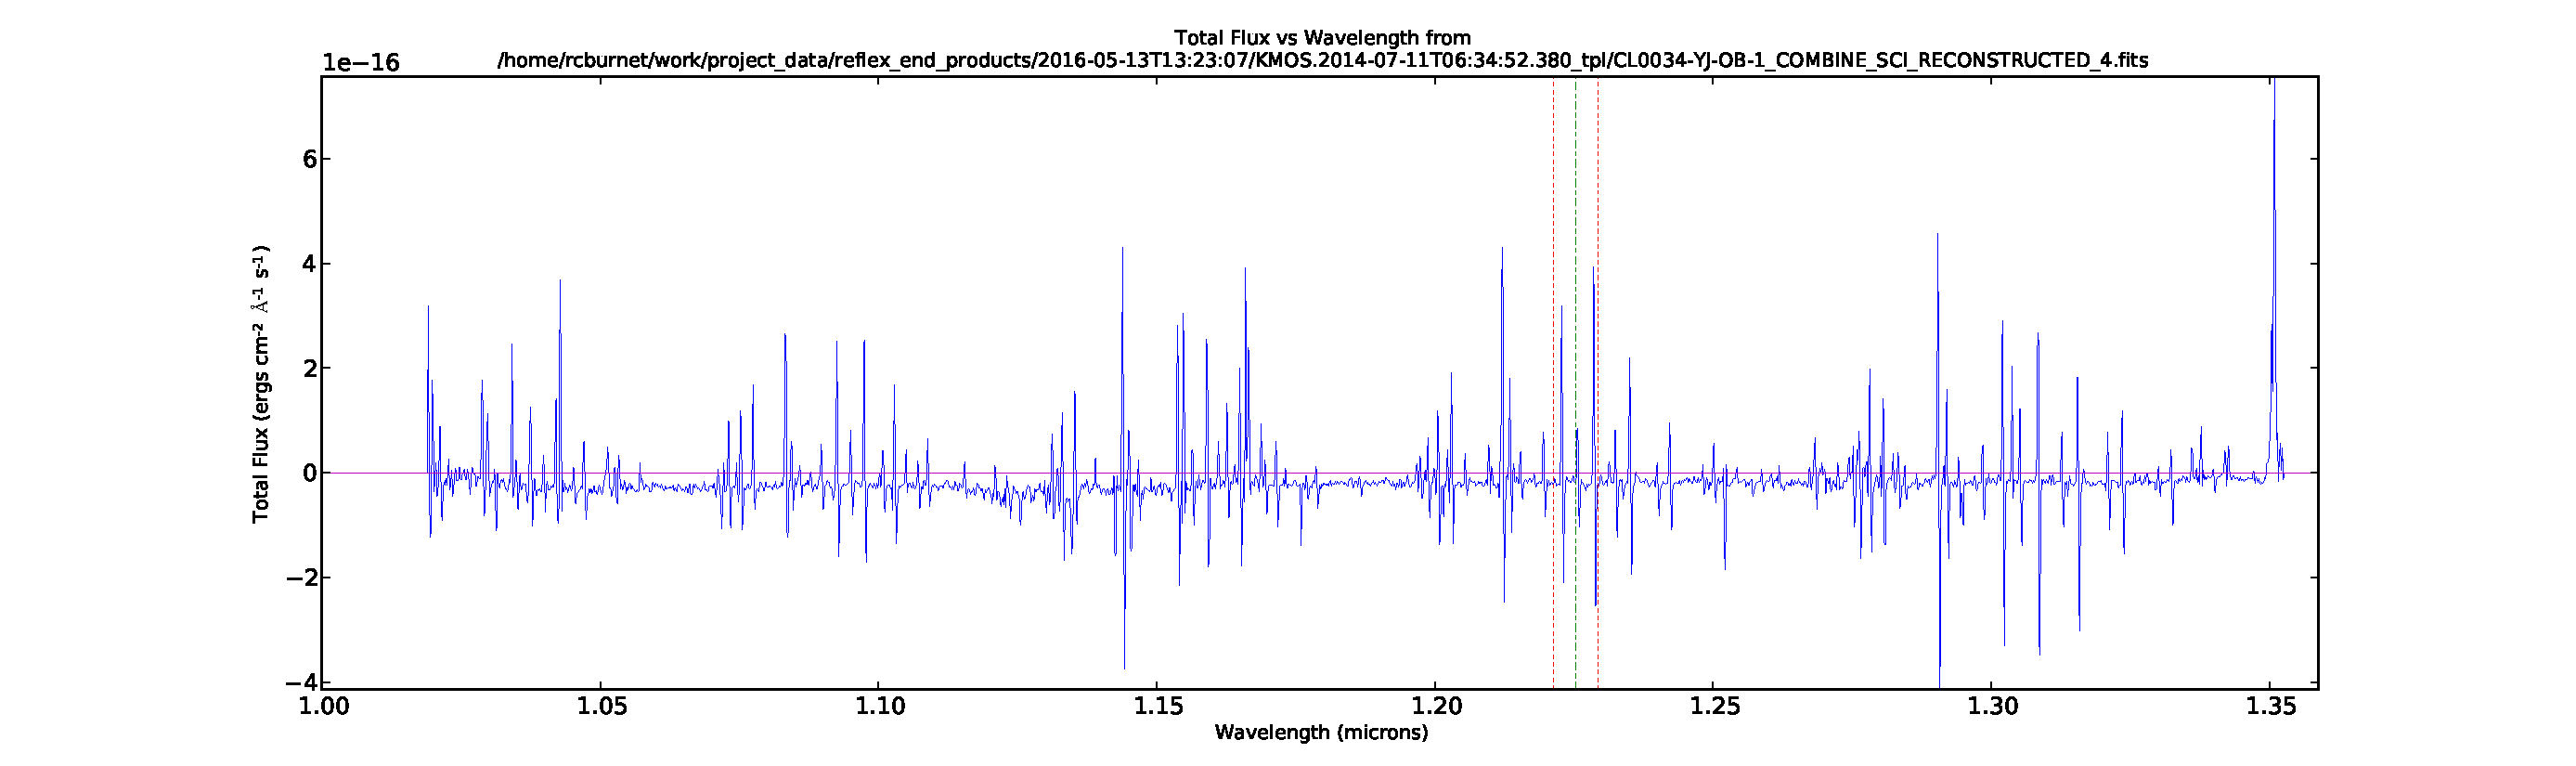
\includegraphics[scale=0.4]{figures/CL0034-YJ-OB-1_COMBINE_SCI_RECONSTRUCTED_4.pdf}
\end{figure}
%CL0034-YJ-OB-1_COMBINE_SCI_RECONSTRUCTED_4.fits.pdf

We then plotted the object's sky arm spectrum for each of the interim sky data cubes and overlaid it on top of one of the spectrum of the pre-sky-subtracted interim target data cube. To get the interim data cubes, you had to set the workflow to save the intermediate data. The interim cubes are found in the TMP$\_$PRODUCTS$\_$DIR/kmos$\_$sci$\_$red$\_$1/ directory. But when plotting the spectrum for the object's sky arm flux from each of the interim sky data cubes against its interim target flux (before any sky subtraction), the spikes don't appear at all offset. See the below figure. Note that the flux units are meaningless, this plot is just to see the relative location of the spikes in each of the interim data cubes. The flux from each data cube is scaled to one another so that they all are at the same approximate flux to easily differentiate the spikes. Also note that the data was taken in nod-to-sky mode in sequence ABAAB where A denotes a science frame and B denotes a sky frame. There are two raw sky frames, but 3 interim sky data cubes. The reason being is that the  
pipeline created one sky data cube for each of the three science  
frames, picking the sky frame that was closest in time to each object  
frame. The pipeline made two of the same interim sky data cubes because they each correspond to a different interim object data cube. The first two science frames are subtracted with the first sky frame. Therefore, the first two sky spectrum plots (Sky 2014-09-11T06:34:52.380 and Sky 2014-07-11T06:50:52.037) are the same plots.\\

\begin{figure}[h!]
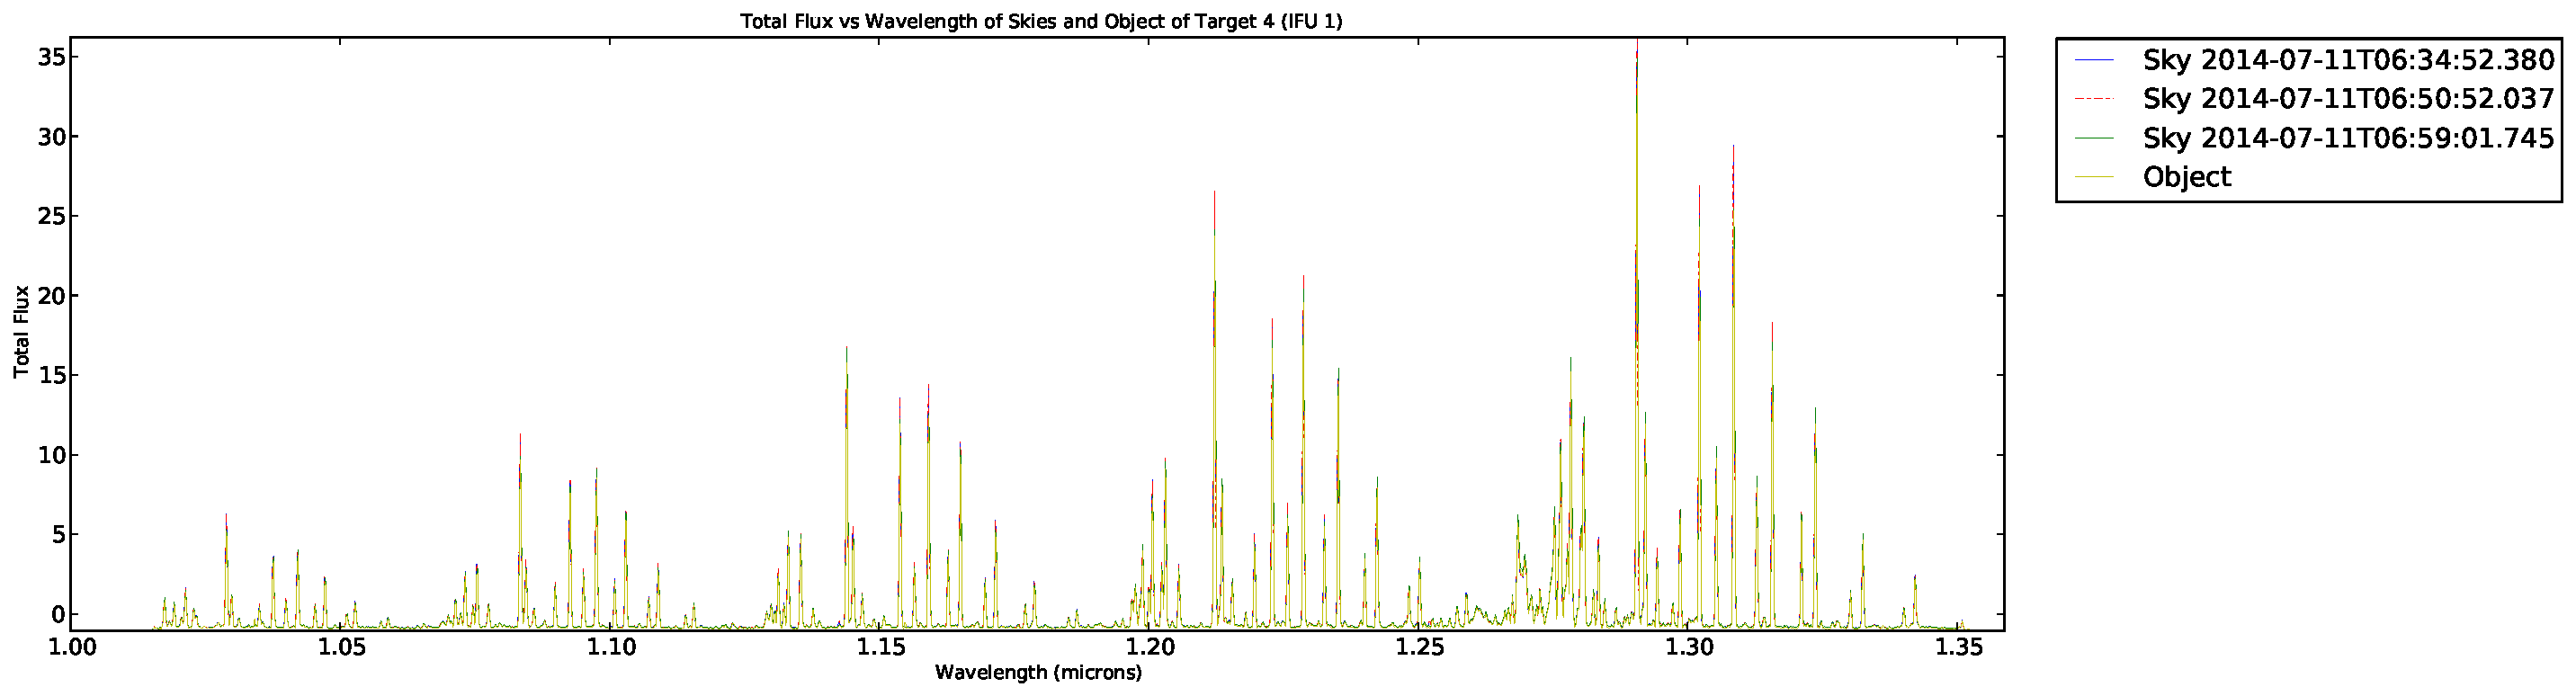
\includegraphics[scale=0.4]{figures/flux_of_target_4_IFU_1_relative_residuals_from_interim_data.pdf}
\end{figure}
%flux_of_target_4_IFU_1_relative_residuals_from_interim_data.pdf

We then plotted the relative residuals of the skies from their average, and the relative residuals of the object flux from it's average flux, for each interim object and sky frame, for object 4. By relative residuals, I mean I subtracted each sky and object flux from the average flux of the skies at each wavelength slice. This time, I used only two sky interim data cubes (since 2 of the three are the same, it's unnecessary to use all three) and plotted the spectrum for all 3 interim object data cubes, using the observation times of the data cubes corresponding raw data frames to distinguish between them in the legend. See figure below.\\

\begin{figure}[h!]
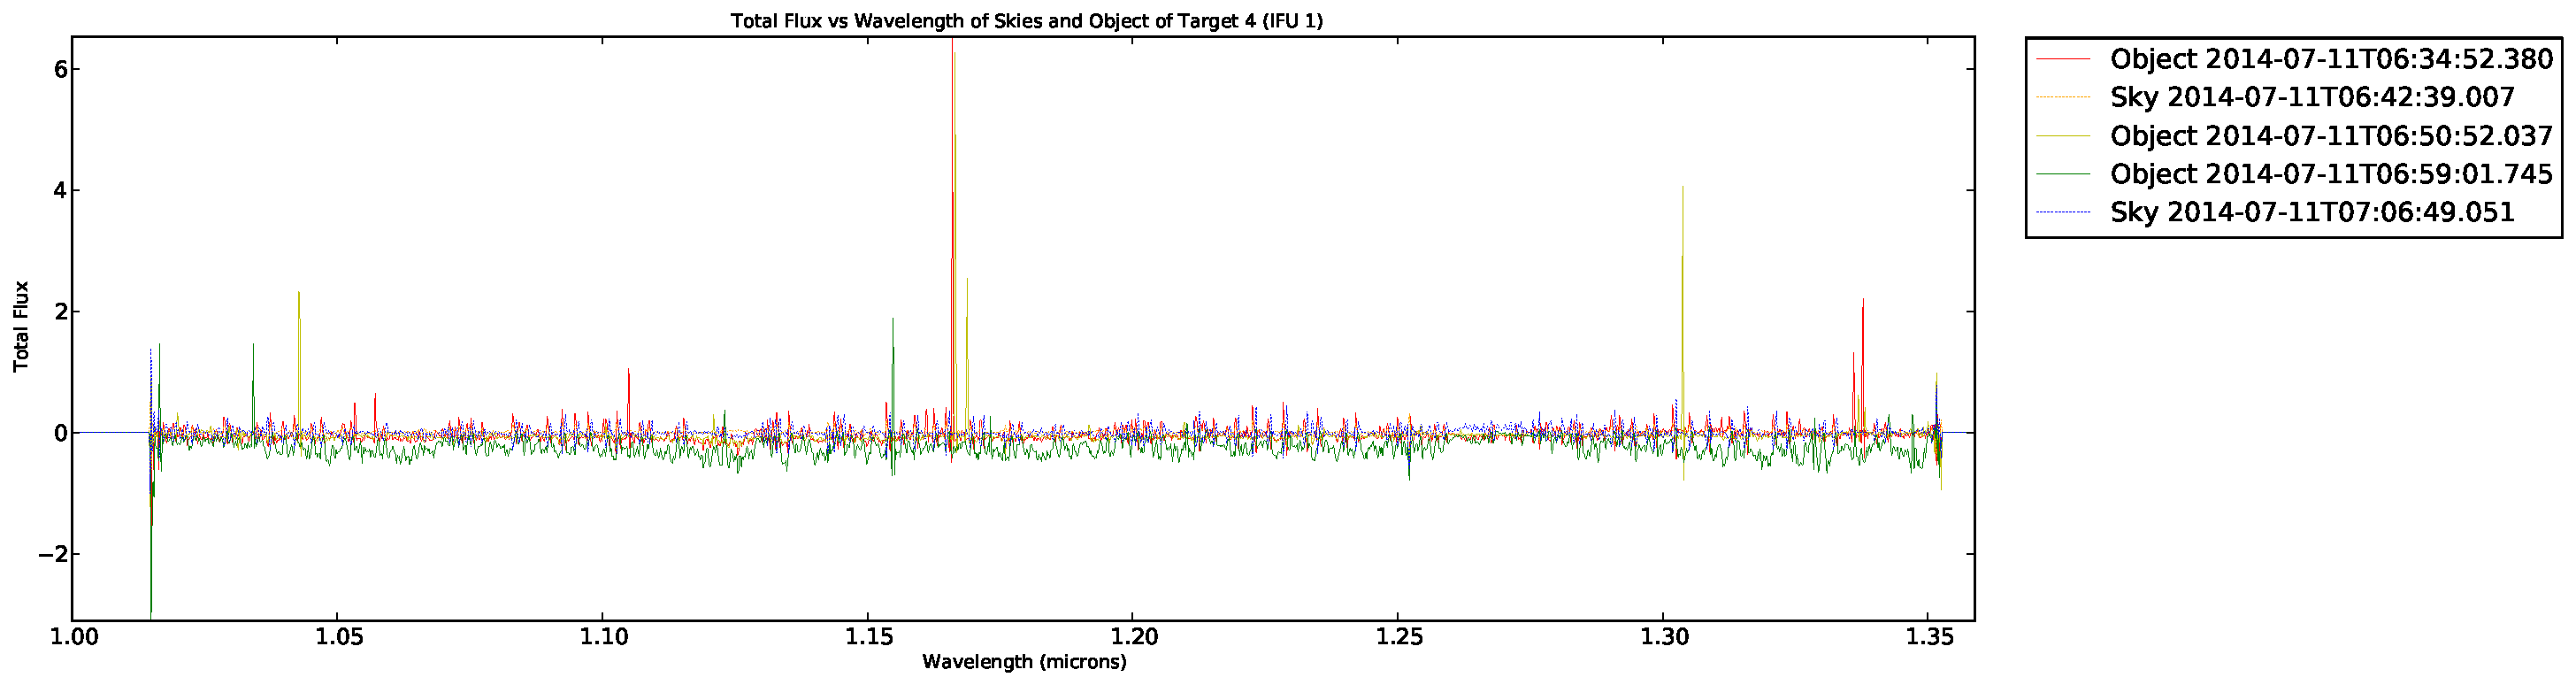
\includegraphics[scale=0.4]{figures/sky_flux_raw.pdf}
\end{figure}
%sky_flux_raw.pdf

We noted that the third object data cube (Object 2014-07-11T06:59:01.745) had less flux than the others and also seemed noisier. Perhaps a cloud got in the way during the observation of that frame? We then checked to see if it was consistent with the other objects (ie. was it always the third frame that had less flux and was noisier?), but that wasn't the case as you can see in the figure below of the relative residuals of object 11. This time, the third frame had greater flux than the skies.\\

\begin{figure}[h!]
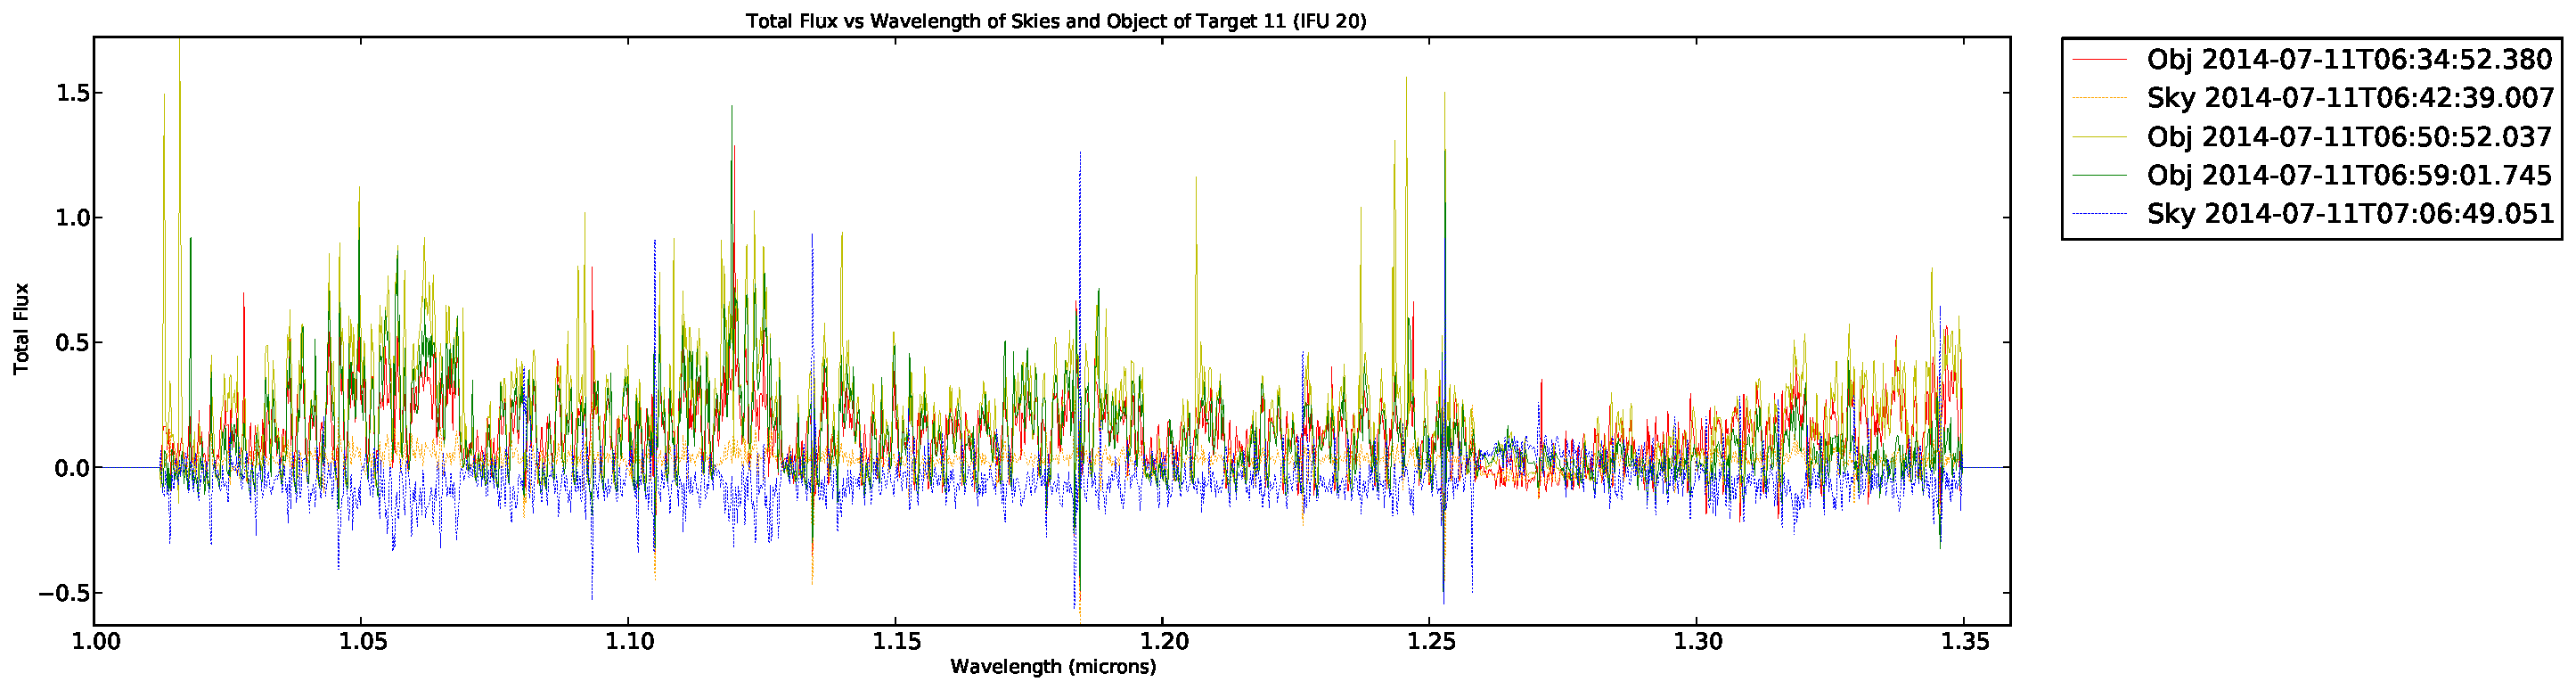
\includegraphics[scale=0.4]{figures/sky_flux.pdf}
\end{figure}
%sky_flux.pdf

The above three plots were generated from ``sky$\_$subtraction$\_$look.py. The script now only generates the plots of the relative residuals of the skies from their average, and the relative residuals of the object flux from it's average flux, for each interim object and sky frame.\\

\section{Laptop work}
I switched to work on a laptop with Fedora 23 installed on May 24. No more work was carried out on the desktop. As a result, some directory names will change in the scripts. If you wish to look into them, I've put my work that I've done on my laptop onto the desktop. Be wary of the directory name and designation changes. From here on, the $\sim$ directory will refer to the /home/rburnet/ directory on my laptop (/home/rcburnet/ on desktop).

\subsection{May 24: Sean's catalogue, spectrum of specific targets, spectrum of specific targets' specific spaxels}
It was at this point I learned that some of the IFUs in the object frame were pointing at sky, as if they were in stare mode, but the data was clearly in nod-to-sky mode with the ABAAB frames and the pipeline handled the data as if it were in nod-to-sky mode. As a result, the pipeline completely ignored the IFUs in the science frames that were pointing to sky and simply used the sky arms from the sky frames to carry out sky subtraction of their corresponding target arms from the science frames. Specifically, arms 2 (origarm 4) and 5 (origarm 7) for CL0034 in YJ-band and arms 5 (origarm 7), 13 (origarm 15), 17 (origarm 19), and 21 (origarm 23) for CL0036 in YJ-band were pointed to sky and thus ignored by the pipeline. Note that origarm corresponds to the original arm name before rotator optimization (as detailed in the primary headers of the raw data frames and pipeline reduced data cubes) where as arm simply refers to the IFU arm name. They are not the same.\\

Balogh provided me with Sean's catalogue of the targets in the KMOS datasets, which had details such as the targets' redshifts, magnitudes, SFR(OII) values, and other relevant information. See the table below.\\

%Sean's catalogue table

We then looked at target 5 (origarm 10, highest SFR(OII)) and target 11 (origarm 22, brightest target in cluster) from CL0034 and target 4 (origarm 2, highest SFR(OII)) and target 15 (origarm 11, brightest target in cluster) from CL0036 as they were detailed in Sean's catalogue as targets with large SFR(OII) values and small magnitudes (brighter sources), which would mean we'd expect the most H$\alpha$ flux from these targets and a detection of continuum. We plotted their spectrum with the pipeline's default parameters with the exact location we'd expect the H$\alpha$ line and NII lines to appear with the given target's redshift (as detailed in Sean's catalogue). See script $\sim$/S16work/total$\_$flux$\_$vs$\_$wavelength$\_$scripts/total$\_$flux$\_$vs$\_$wavelength$\_$specific.py. See the figures below.\\

\begin{figure}[h!]
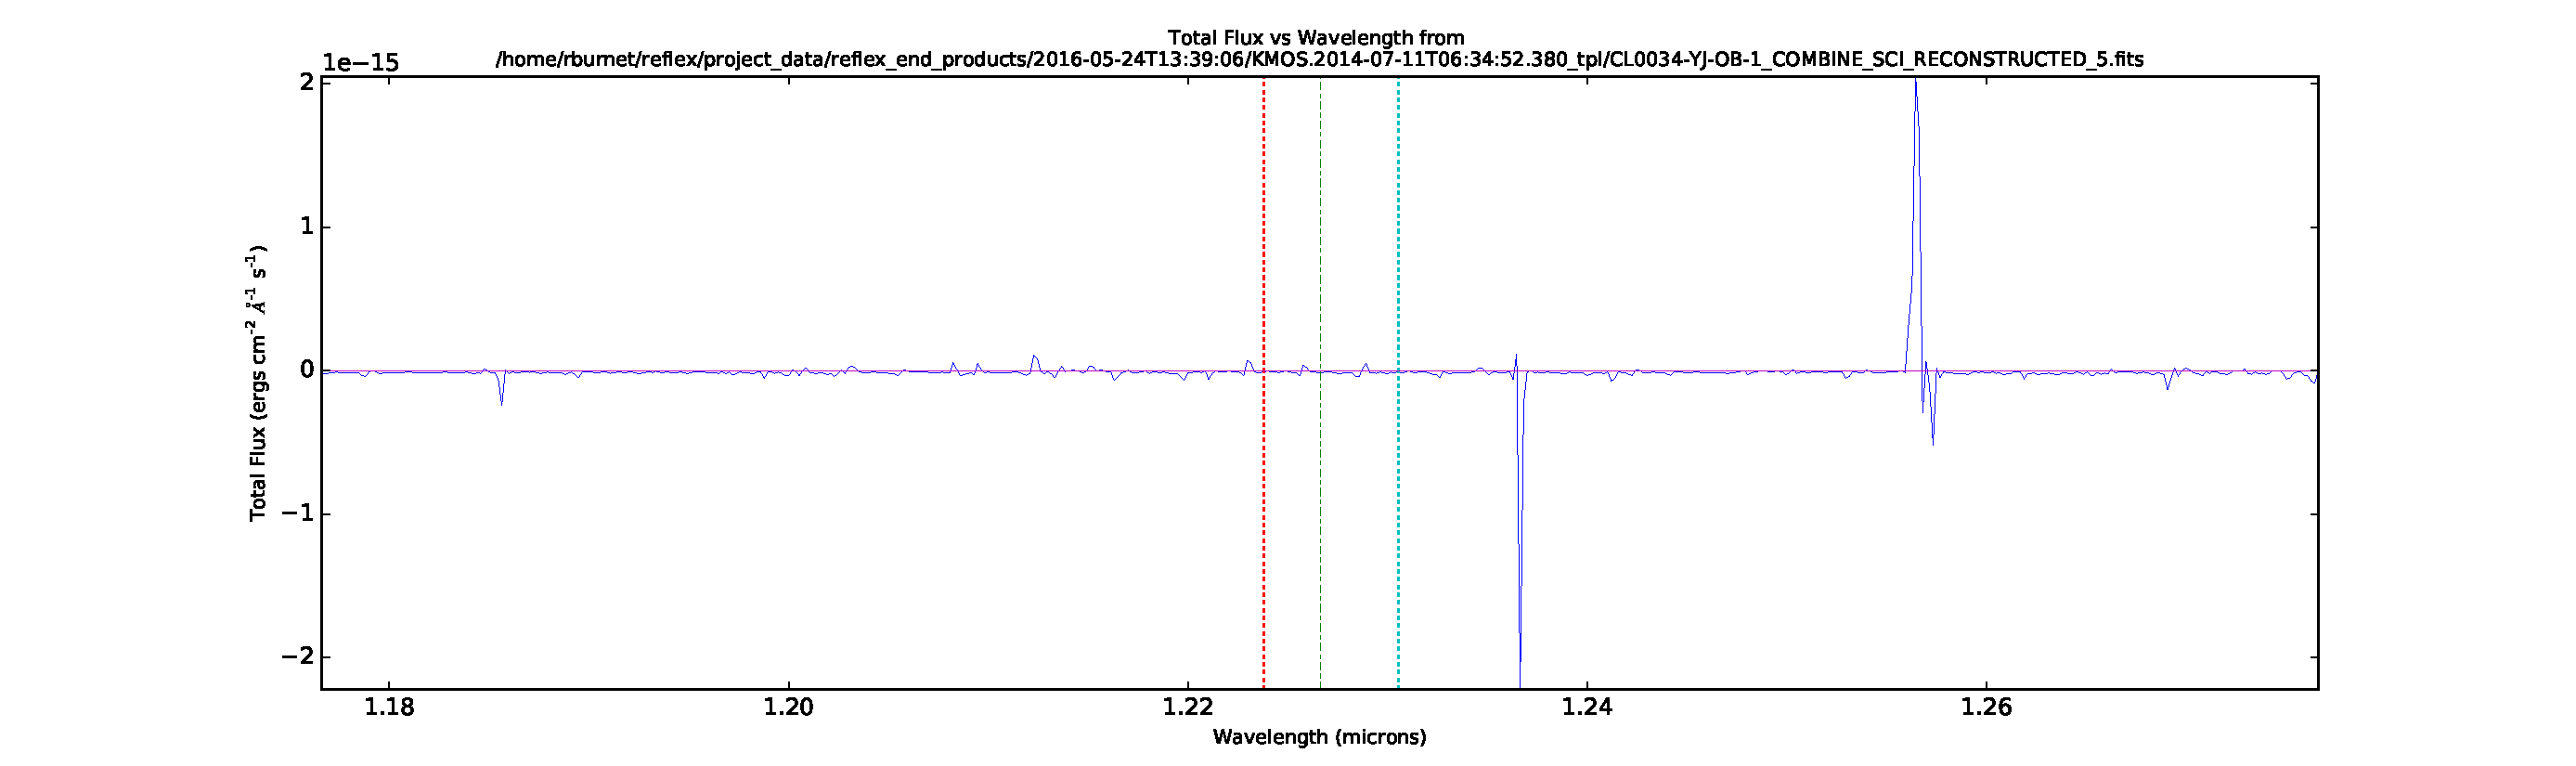
\includegraphics[scale=0.4]{figures/CL0034-YJ-OB-1_COMBINE_SCI_RECONSTRUCTED_5.pdf}
\end{figure}
%/home/rburnet/S16work/formal_documentation/figures/CL0034-YJ-OB-1_COMBINE_SCI_RECONSTRUCTED_5.fits.pdf
\begin{figure}[h!]
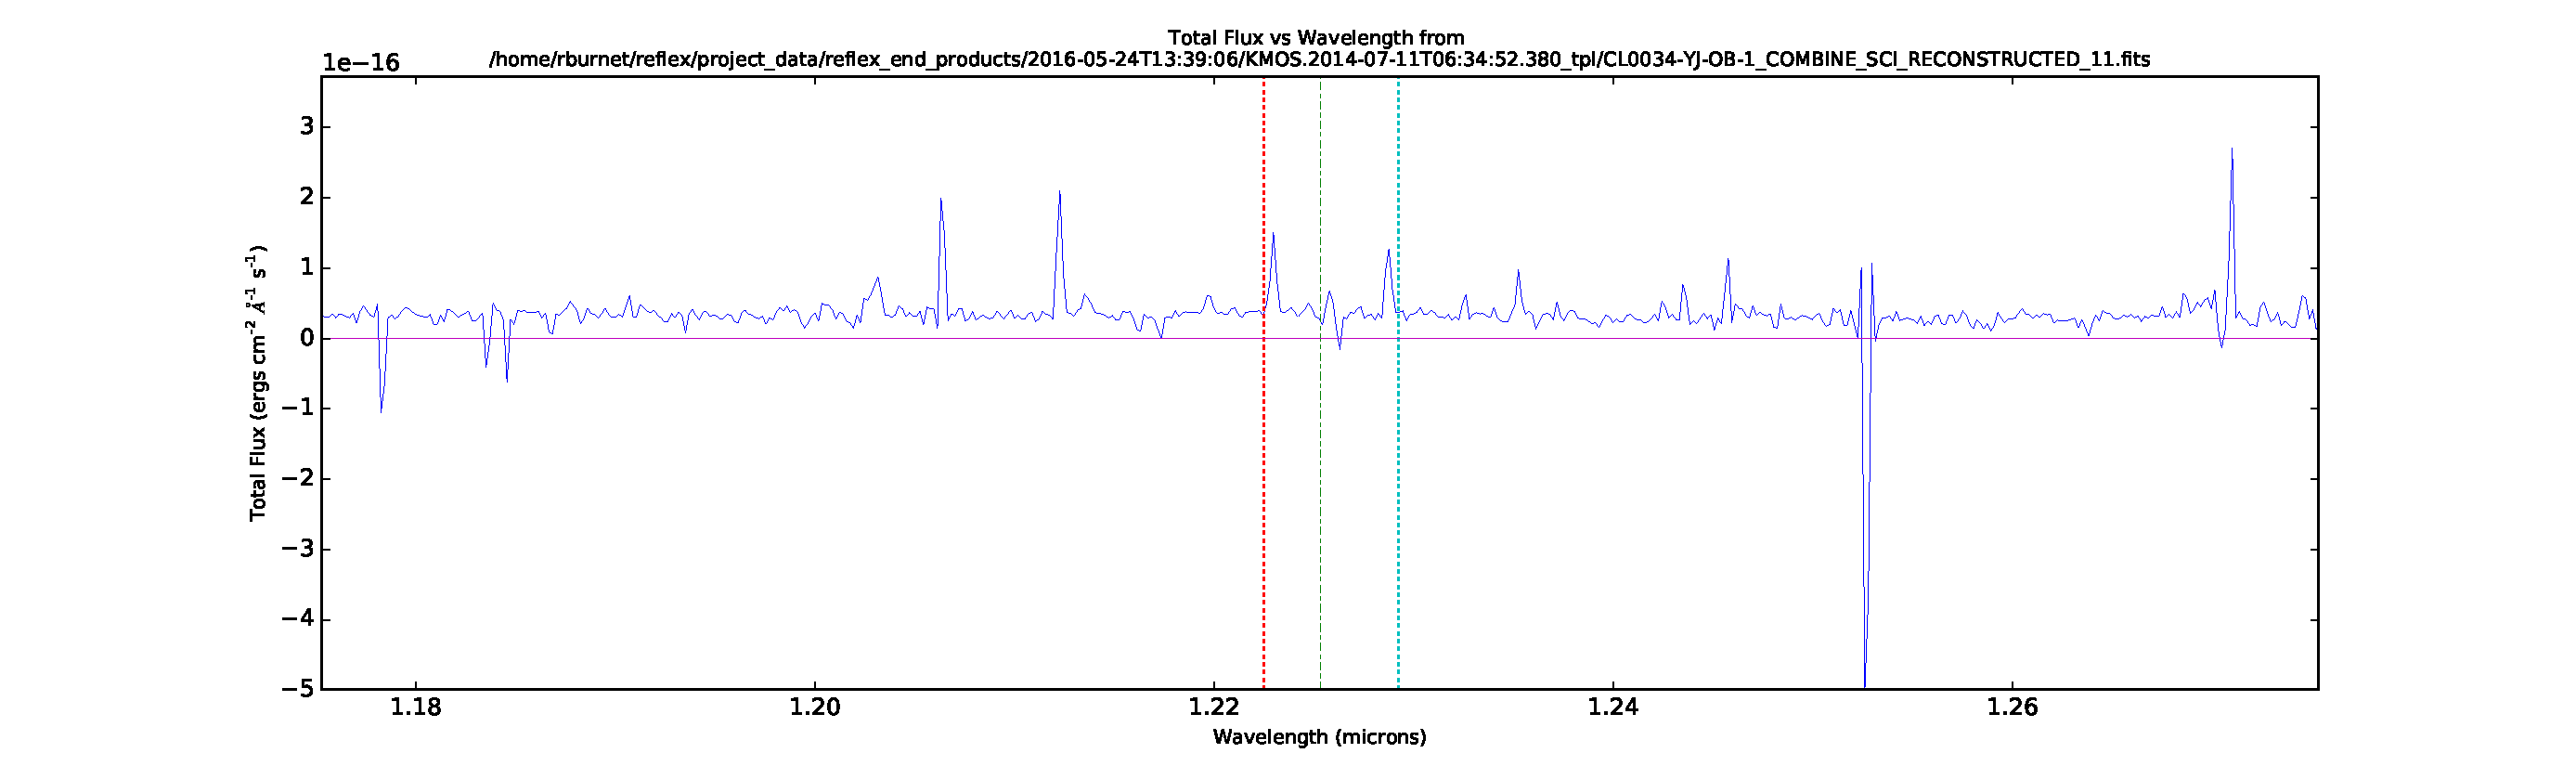
\includegraphics[scale=0.4]{figures/CL0034-YJ-OB-1_COMBINE_SCI_RECONSTRUCTED_11.pdf}
\end{figure}
%/home/rburnet/S16work/formal_documentation/figures/CL0034-YJ-OB-1_COMBINE_SCI_RECONSTRUCTED_11.fits.pdf
\begin{figure}[h!]
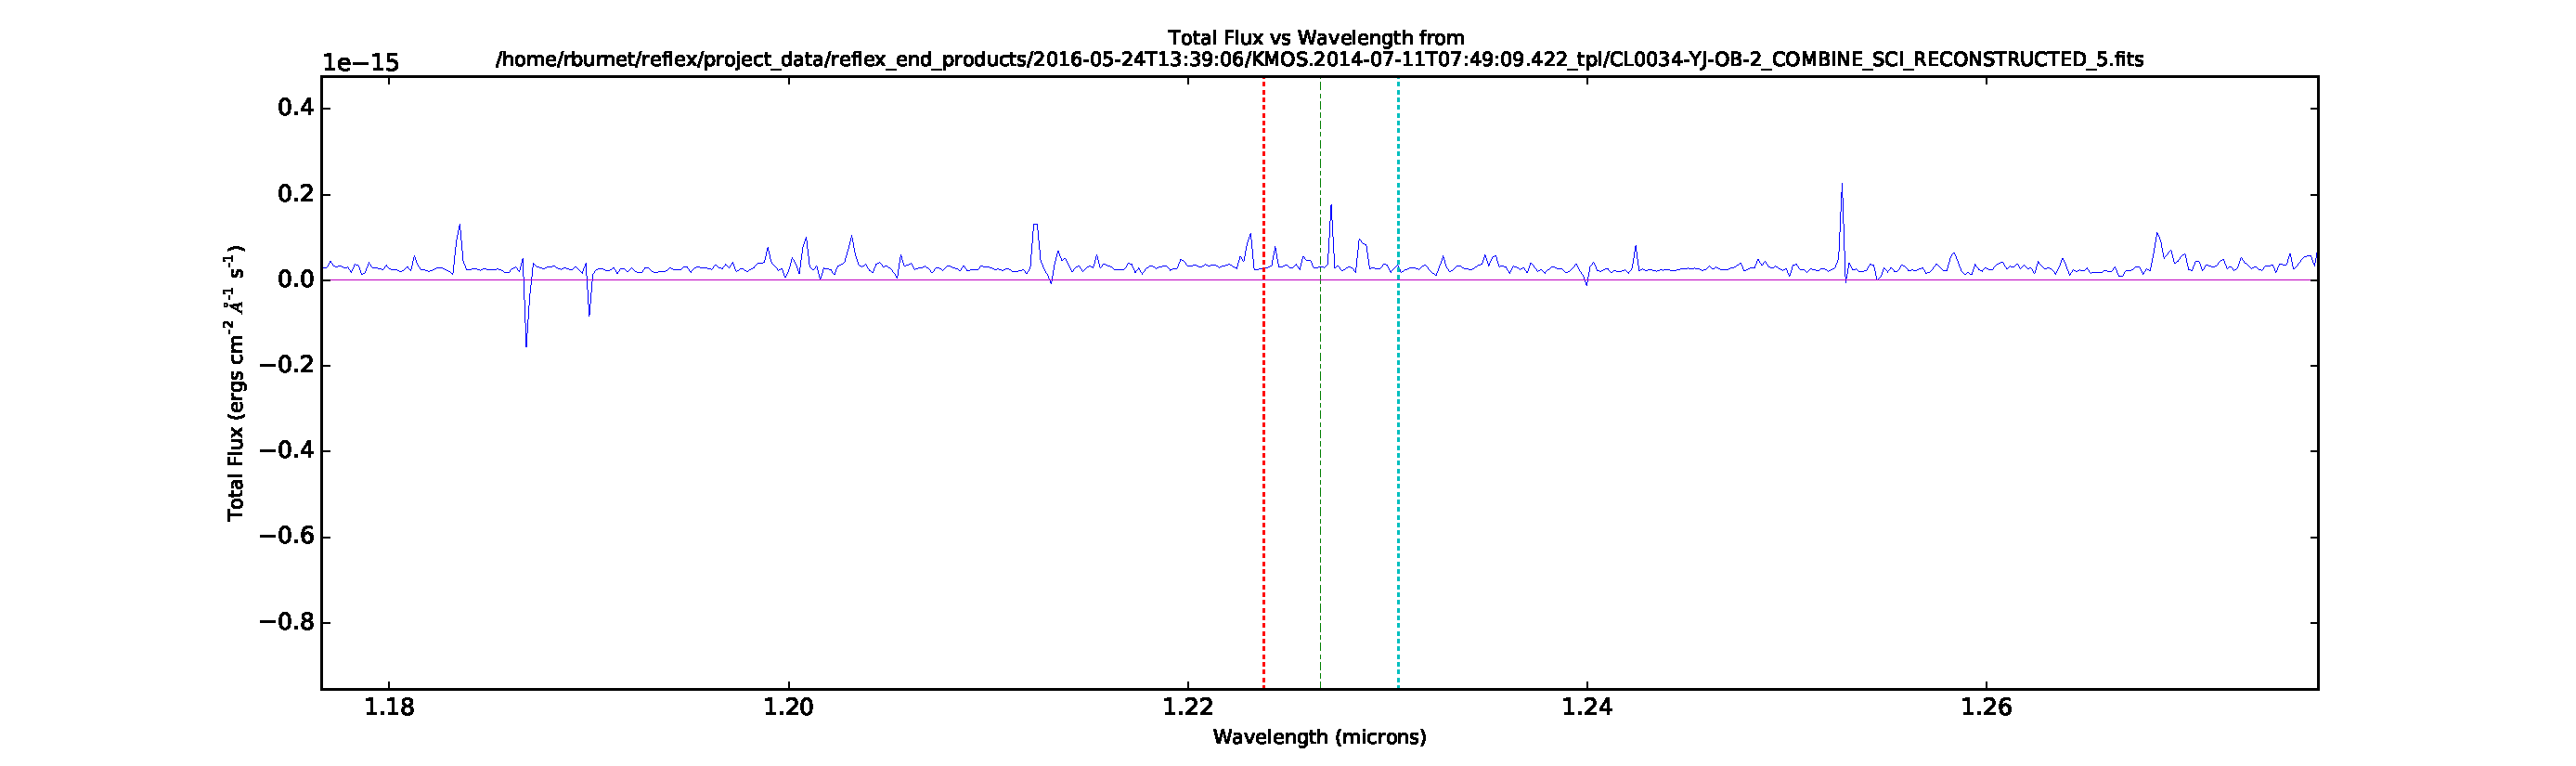
\includegraphics[scale=0.4]{figures/CL0034-YJ-OB-2_COMBINE_SCI_RECONSTRUCTED_5.pdf}
\end{figure}
%/home/rburnet/S16work/formal_documentation/figures/CL0034-YJ-OB-2_COMBINE_SCI_RECONSTRUCTED_5.fits.pdf
\begin{figure}[h!]
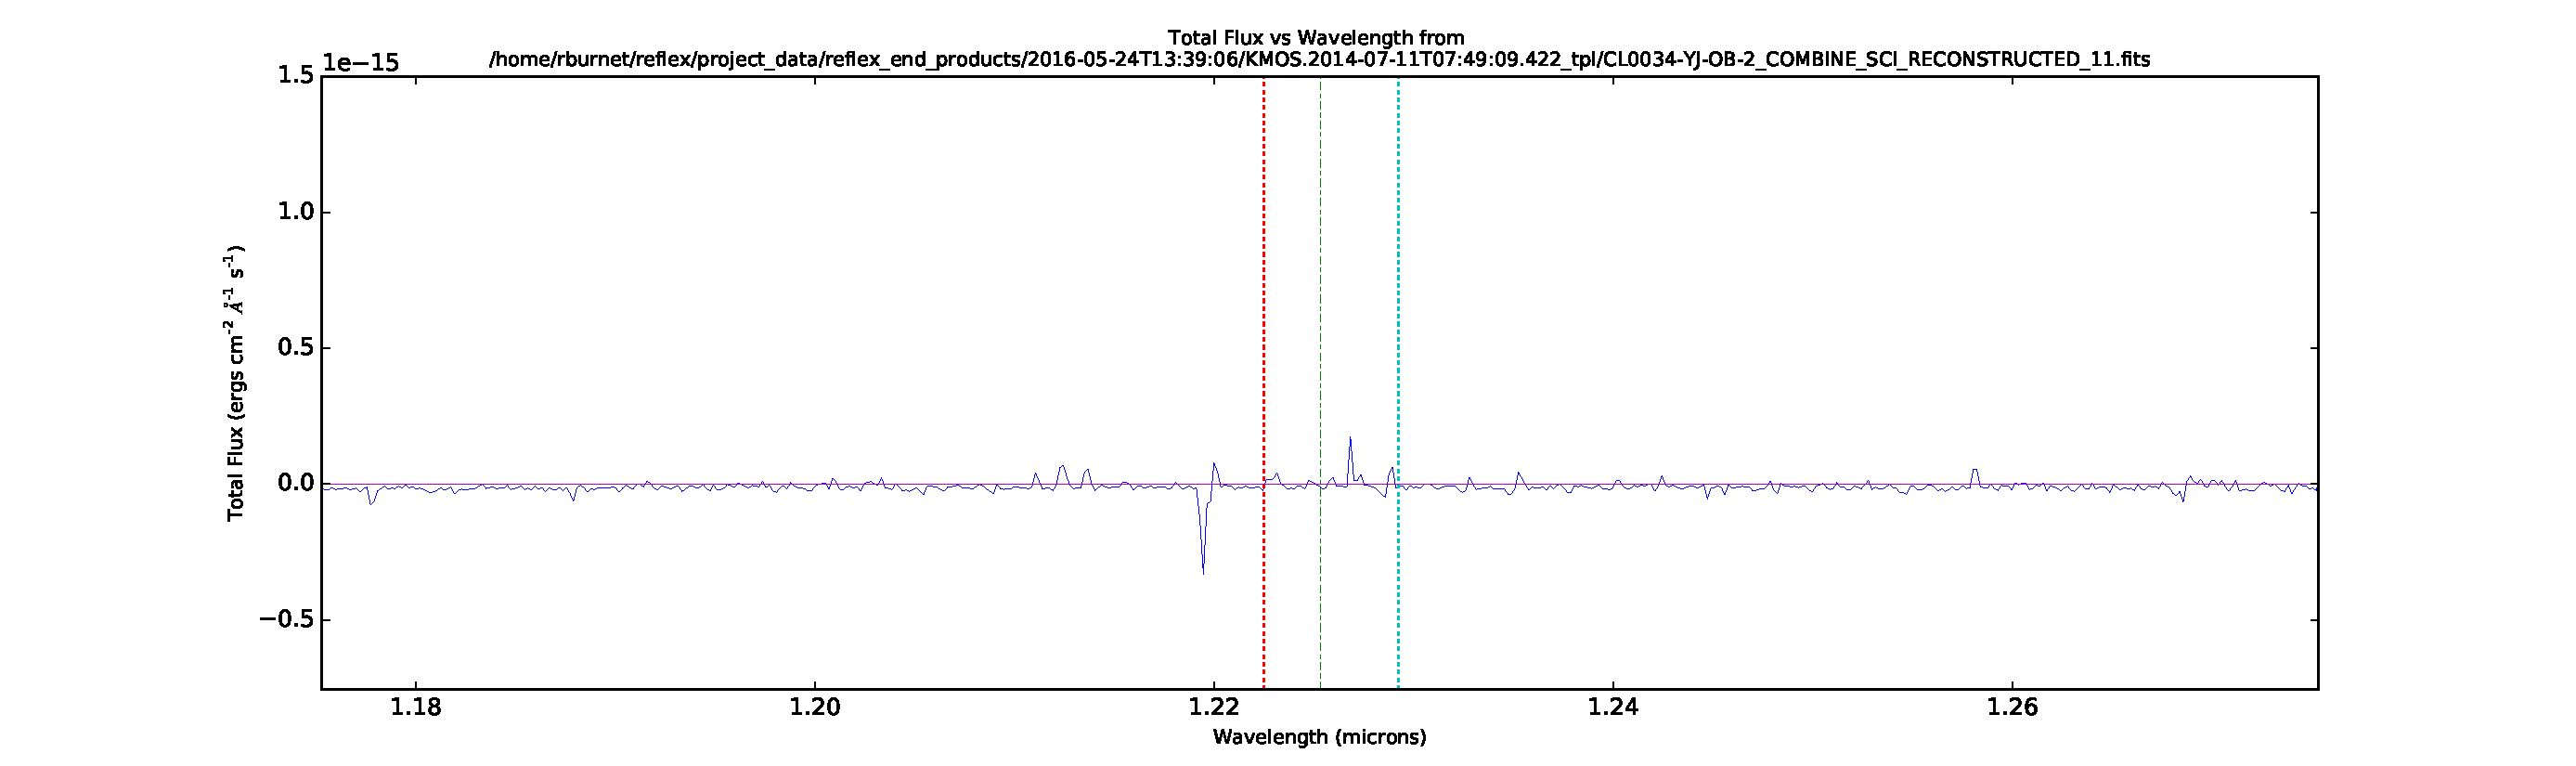
\includegraphics[scale=0.4]{figures/CL0034-YJ-OB-2_COMBINE_SCI_RECONSTRUCTED_11.pdf}
\end{figure}
%/home/rburnet/S16work/formal_documentation/figures/CL0034-YJ-OB-2_COMBINE_SCI_RECONSTRUCTED_11.fits.pdf
\begin{figure}[h!]
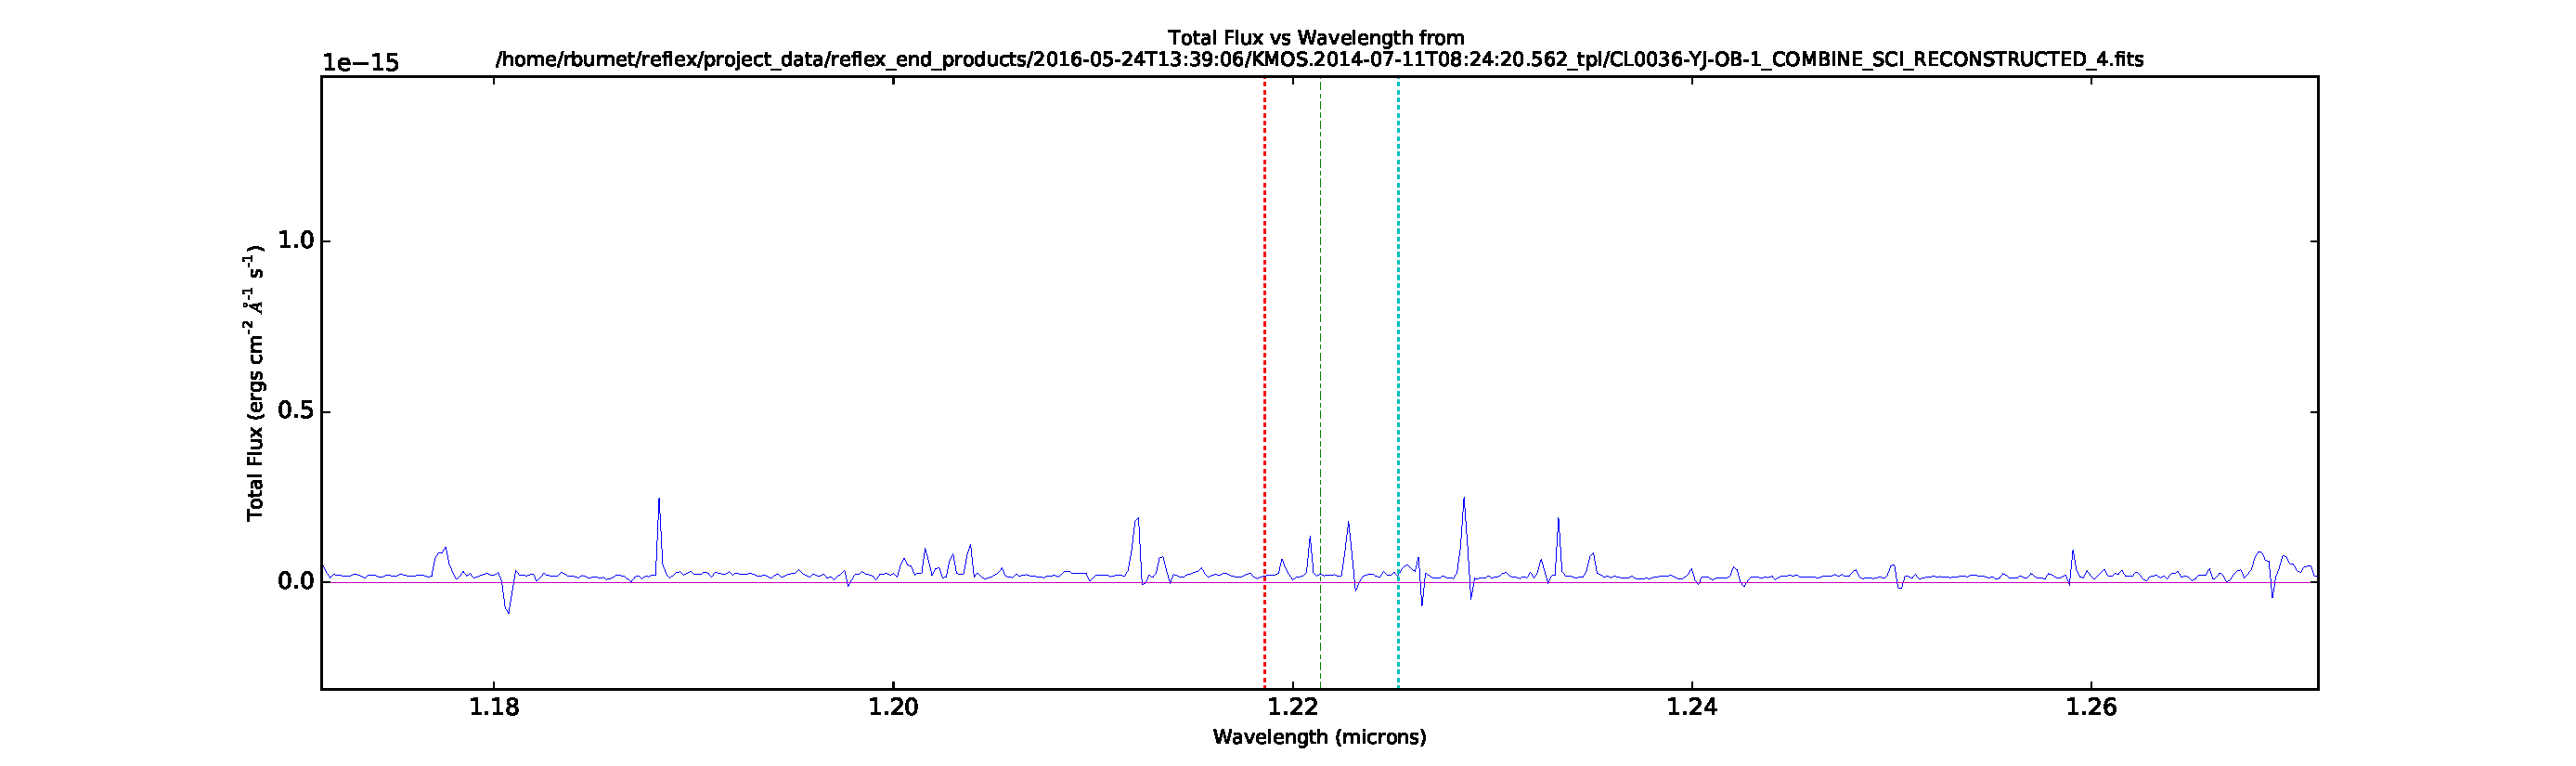
\includegraphics[scale=0.4]{figures/CL0036-YJ-OB-1_COMBINE_SCI_RECONSTRUCTED_4.pdf}
\end{figure}
%/home/rburnet/S16work/formal_documentation/figures/CL0036-YJ-OB-1_COMBINE_SCI_RECONSTRUCTED_4.fits.pdf
\begin{figure}[h!]
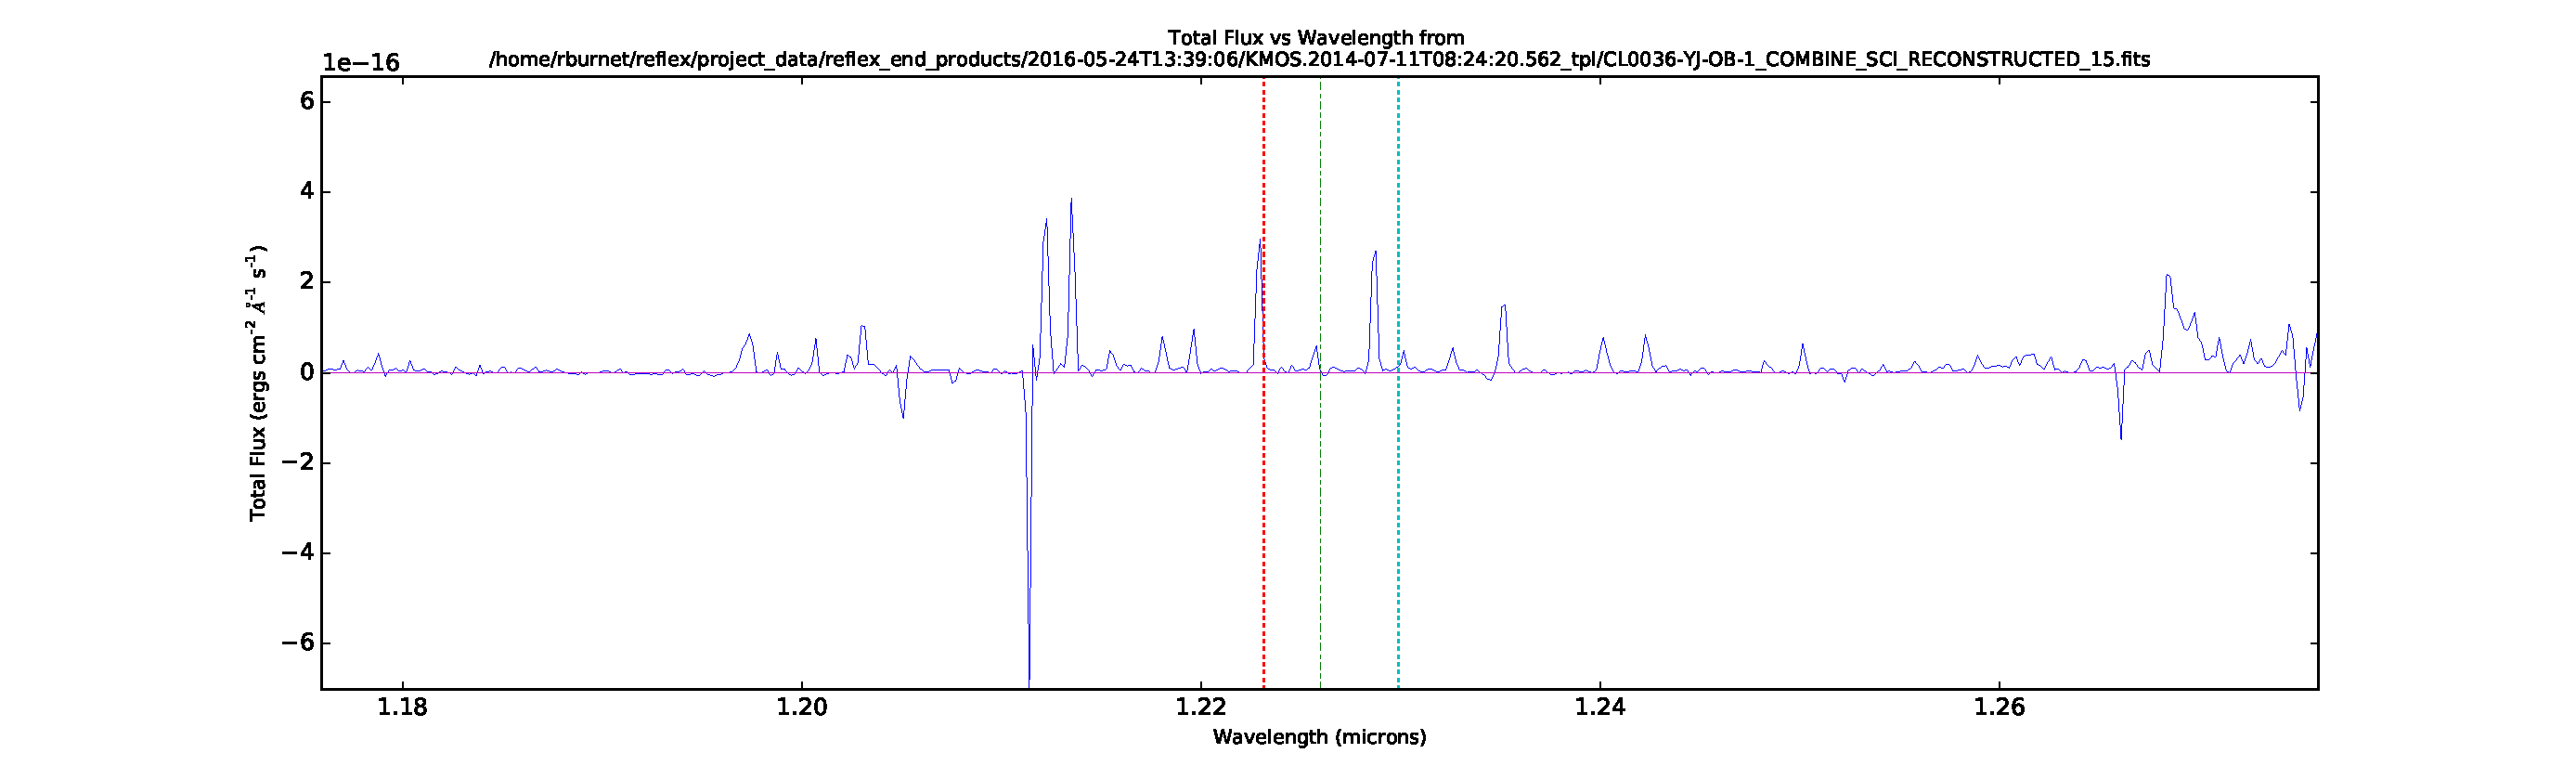
\includegraphics[scale=0.4]{figures/CL0036-YJ-OB-1_COMBINE_SCI_RECONSTRUCTED_15.pdf}
\end{figure}
%/home/rburnet/S16work/formal_documentation/figures/CL0036-YJ-OB-1_COMBINE_SCI_RECONSTRUCTED_15.fits.pdf
\begin{figure}[h!]
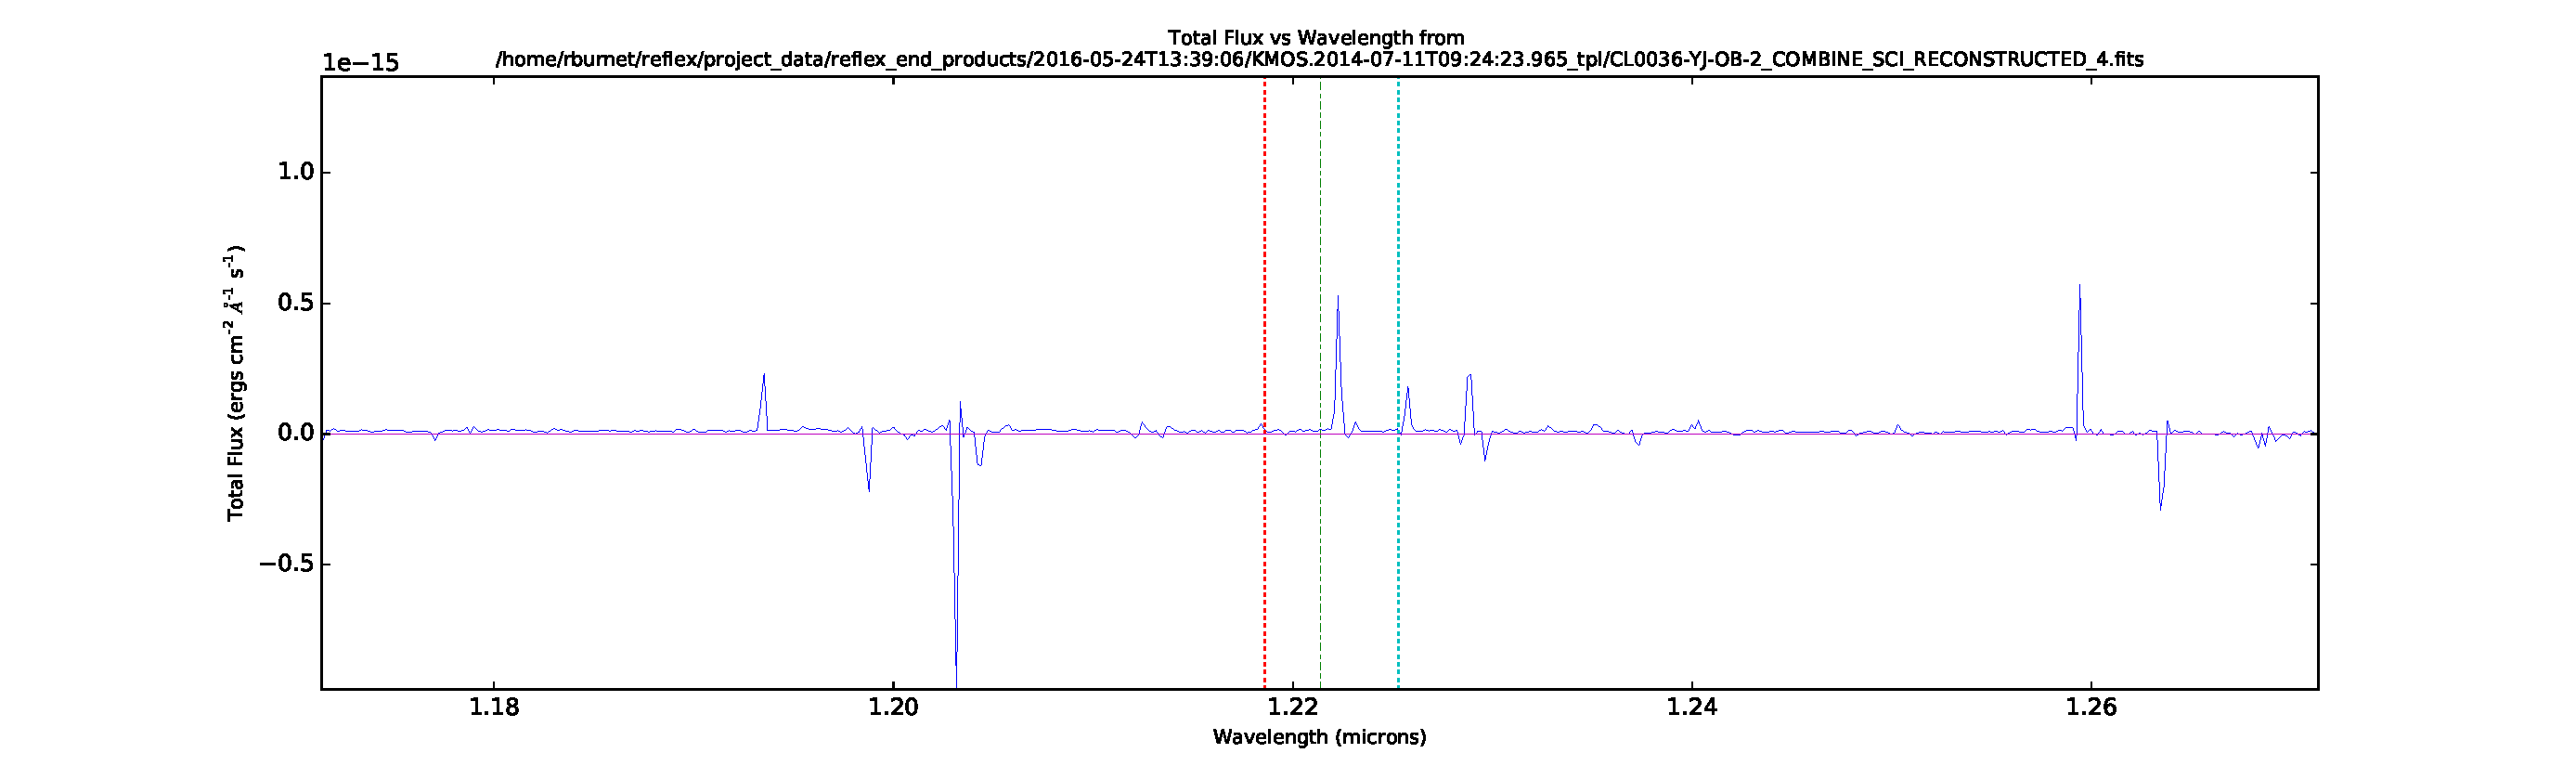
\includegraphics[scale=0.4]{figures/CL0036-YJ-OB-2_COMBINE_SCI_RECONSTRUCTED_4.pdf}
\end{figure}
%/home/rburnet/S16work/formal_documentation/figures/CL0036-YJ-OB-2_COMBINE_SCI_RECONSTRUCTED_4.fits.pdf
\begin{figure}[h!]
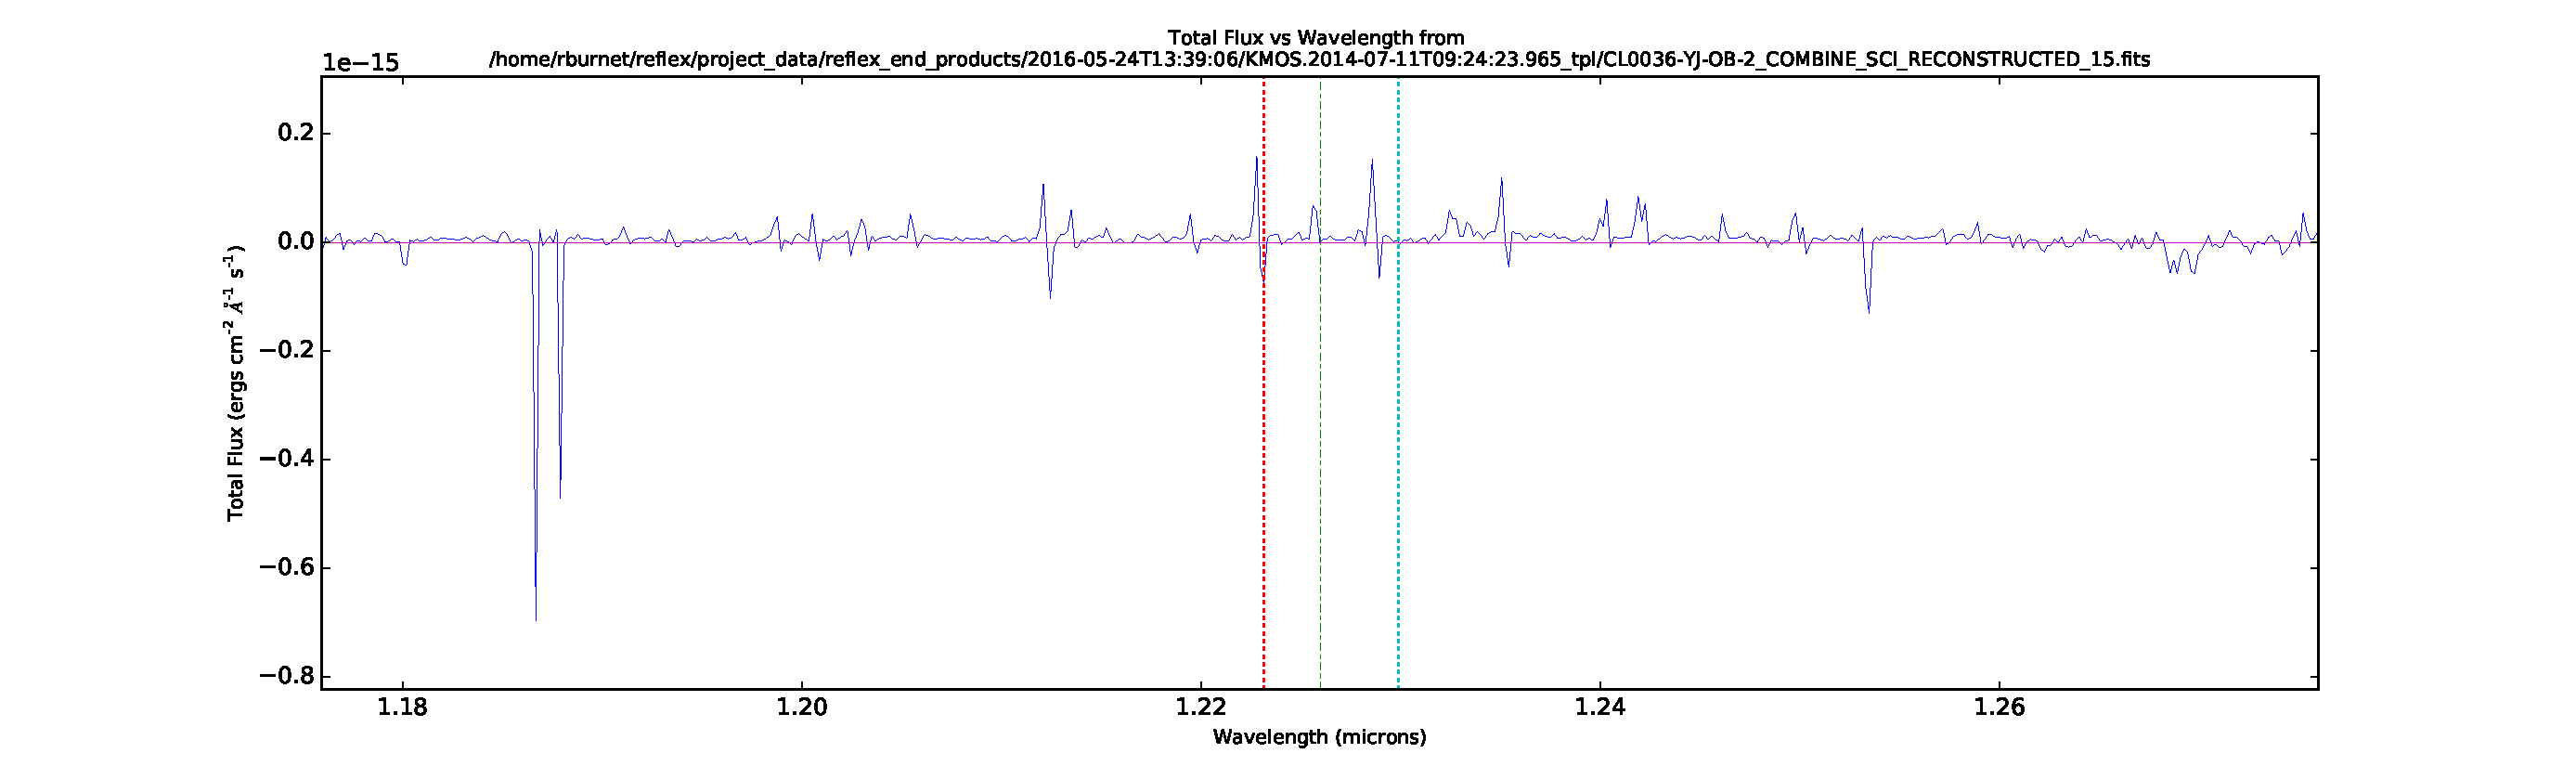
\includegraphics[scale=0.4]{figures/CL0036-YJ-OB-2_COMBINE_SCI_RECONSTRUCTED_15.pdf}
\end{figure}
%/home/rburnet/S16work/formal_documentation/figures/CL0036-YJ-OB-2_COMBINE_SCI_RECONSTRUCTED_15.fits.pdf
\hspace{1cm} \\
\hspace{1cm} \\
\hspace{1cm} \\

But still, no H$\alpha$ detection. Note: OB1 refers to observation block 1 (ABAAB sequence) whereas OB2 refers to observation block 2 (ABA sequence). The pipeline did not combine the two observation blocks into one, and instead kept them split and reduced them separately. Before this, I've been only looking at OB1 data instead of OB2 (as it had more exposures), but now I looked at both.\\

When looking at the collapsed images that the pipeline produced, some targets seemed to have sources while others appeared not to. Looking at the collapsed cube of CL0034 Target 11, there appeared to be some hint of a source near the center. See the figure below of the collapsed cube of CL0034 target 11.\\

\begin{figure}[h!]
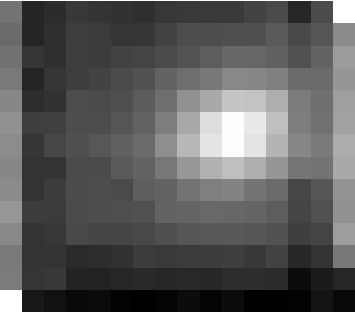
\includegraphics[scale=0.4]{figures/CL0034_target_11_OB1_collapsed.png}
\end{figure}
%/home/rburnet/S16work/formal_documentation/figures/CL0034_target_11_OB1_collapsed.png

I next defined an aperture around the "source" of target 11 (10$<$x$<$14, 4$<$y$<$8) and instead plotted the spectrum of the just the pixels within that aperture to see if there would be any H$\alpha$, but to no avail. 

See script $\sim$/S16work/total$\_$flux$\_$vs$\_$wavelength$\_$scripts/total$\_$flux$\_$vs$\_$wavelength$\_$specific$\_$spaxels.py. See the spectrum below. \\

\begin{figure}[h!]
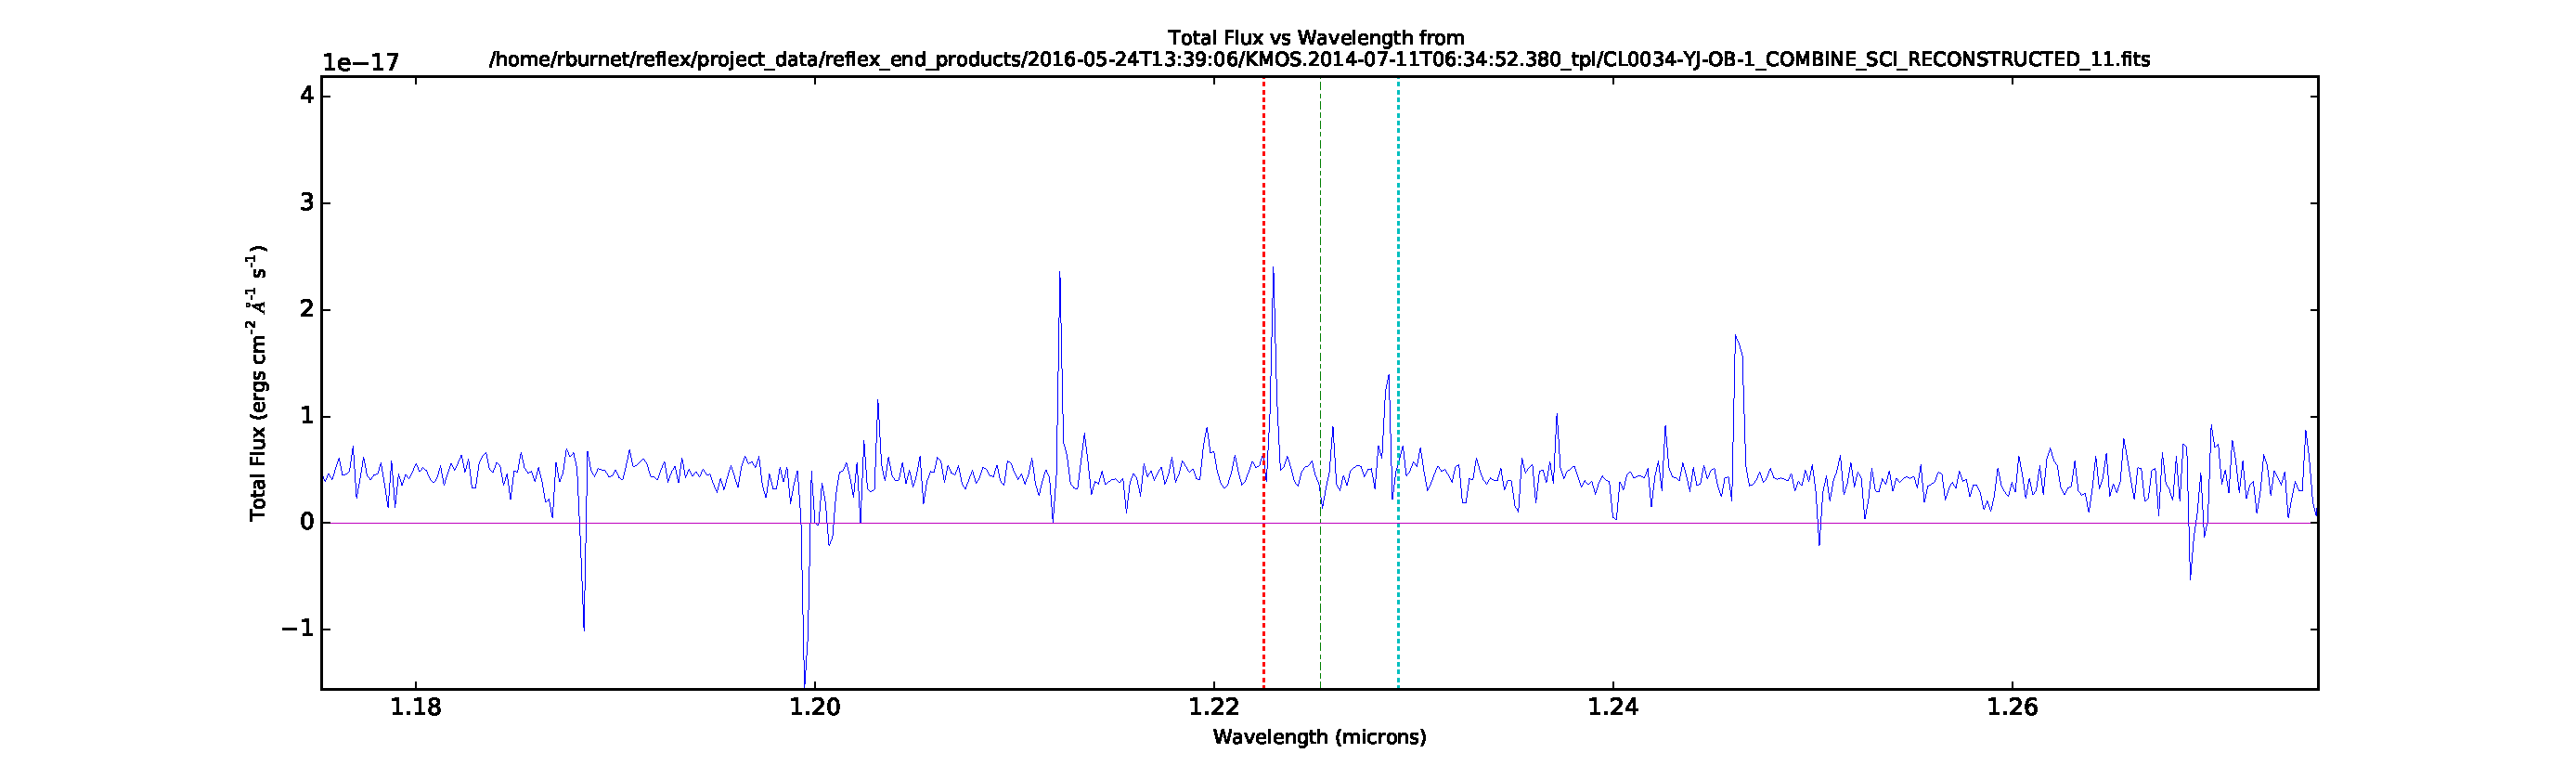
\includegraphics[scale=0.4]{figures/CL0034-YJ-OB-1_COMBINE_SCI_RECONSTRUCTED_11_specific_spaxels.pdf}
\end{figure}
%/home/rburnet/S16work/formal_documentation/figures/CL0034-YJ-OB-1_COMBINE_SCI_RECONSTRUCTED_11_specific_spaxels.fits.pdf

Did the same for CL0036 target 4, with an aperture around the "source" for that target (9$<$x$<$16, 5$<$y$<$12), but again to no avail. See the collapsed image and spectrum of the aperture below.\\

\begin{figure}[h!]

\includegraphics[scale=0.4]{figures/CL0036_target_4_OB1_collapsed.png}
\end{figure}
%/home/rburnet/S16work/formal_documentation/figures/CL0036_target_4_OB1_collapsed.png

\begin{figure}[h!]
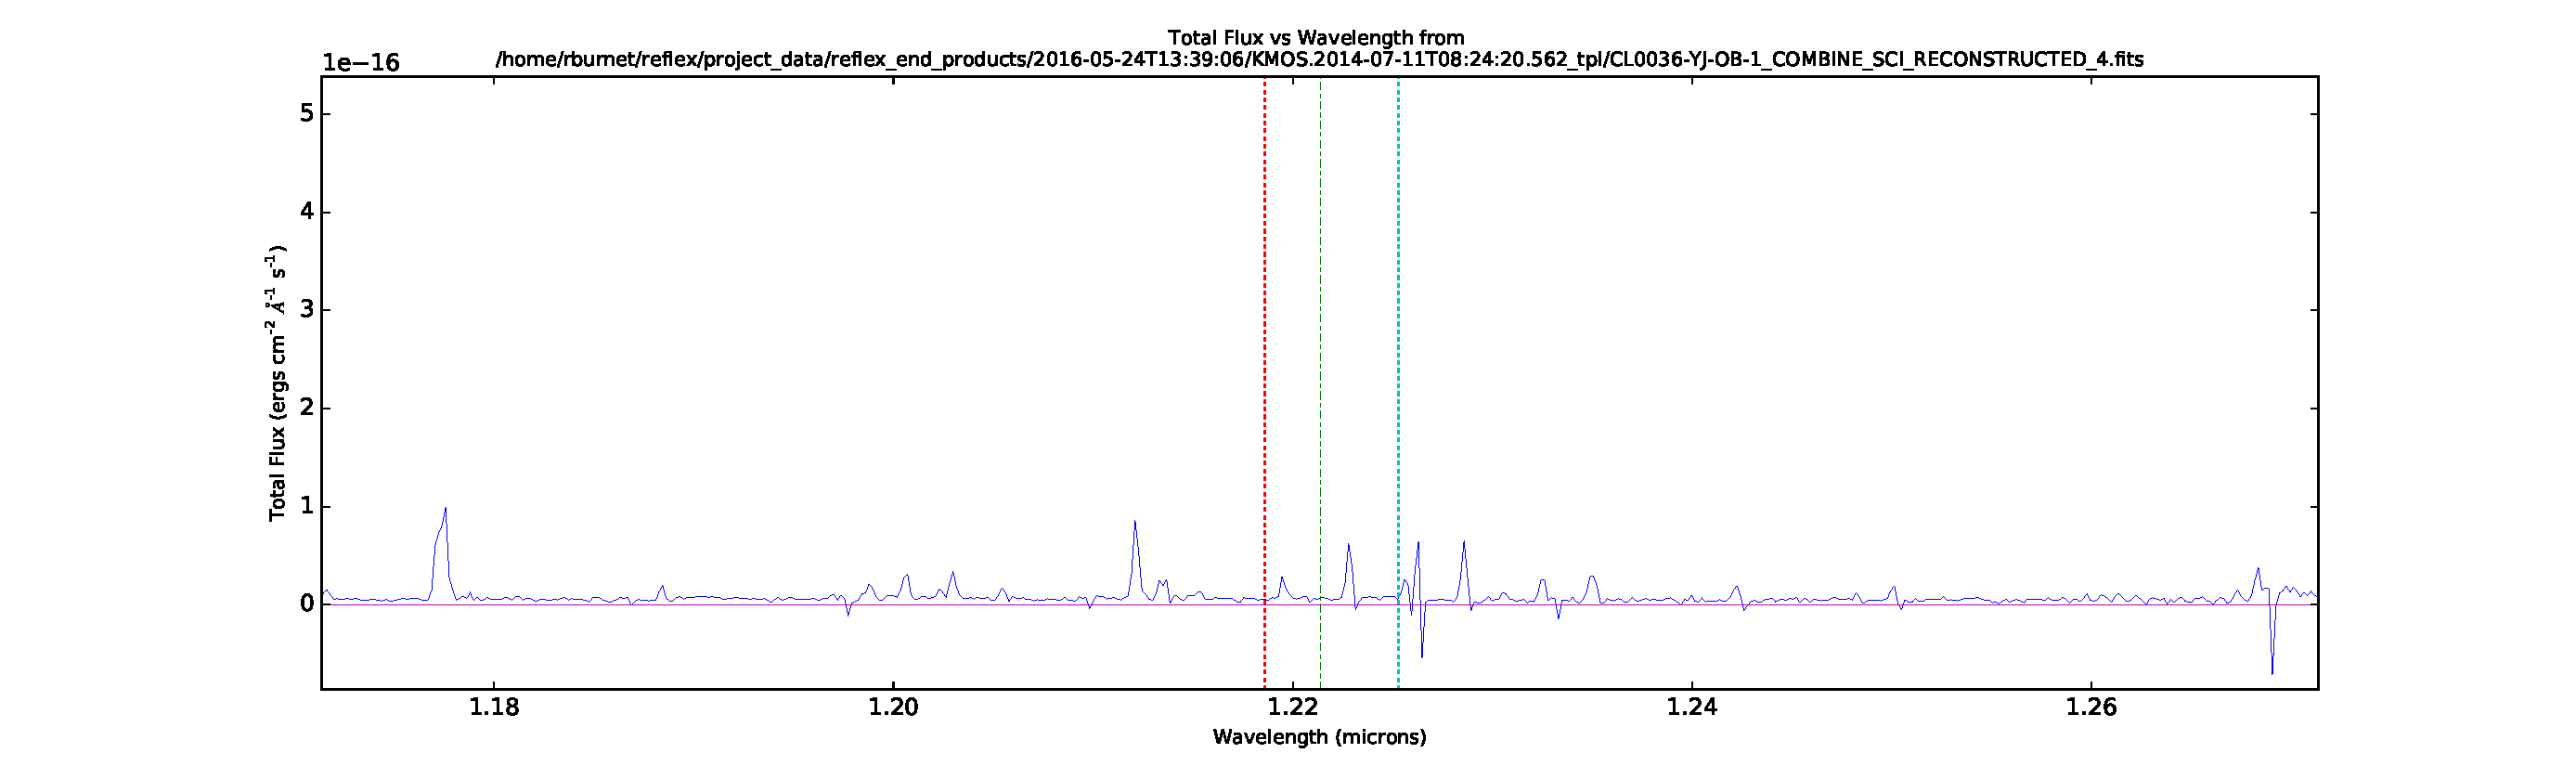
\includegraphics[scale=0.4]{figures/CL0036-YJ-OB-1_COMBINE_SCI_RECONSTRUCTED_4_specific_spaxels.pdf}
\end{figure}
%/home/rburnet/S16work/formal_documentation/figures/CL0036-YJ-OB-1_COMBINE_SCI_RECONSTRUCTED_4_specific_spaxels.fits.pdf

\subsection{May 27: Manual sky subtraction, IZ data cubes}
As the pipeline seemed to not be handling sky subtraction properly, we decided to carry out our own method of sky subtraction on the four targets (two for each cluster) detailed in the last section. You can read up on how the pipeline carries out sky subtraction in document \cite{KMOS pipeline manual}, specifically read up on the kmos$\_$sci$\_$red recipe. Our own method of sky subtraction was the following (see $\sim$/S16work/manual$\_$sky$\_$subtraction$\_$scripts/target$\_$sky$\_$fraction$\_$of$\_$IFU$\_$specific$\_$targets.py):\\

1) Run pipeline workflow with "no subtract" set to true, "sky tweak" set to false, and "save interims" set to true so that the pipeline won't sky subtract the reduced data cubes (both final and intermediate data cubes), allowing us to carry out our own method of sky subtraction.\\

2) Extract the mean perimeter flux at each wavelength slice for each final reduced data cube. Perimeter is defined as the top, bottom, far right, and far left 2 rows/columns so as to be far enough away from the source that we'd expect to be at the center of the cube. Call it T$_{\lambda}$(perimeter).\\

3) Extract mean sky flux from the target's corresponding sky arm final reduced data cube. Call it S$_{\lambda}$(sky).\\

4) Find scaling factor such that:\\
f = $\frac{\text{T}_{\lambda}\text{(perimeter)}}{\text{S}_{\lambda}\text{(sky)}}$\\
to scale the mean sky flux with the mean perimeter target flux, used for scaling the sky spaxels to the target spaxels before sky subtraction.\\

5)Subtract each spaxel of the target cube by it's corresponding sky spaxel from the sky cube scaled by f as:\\
T$\prime _{\lambda}$(spaxel) = T$_{\lambda}$(spaxel) - f $\times$ S$_{\lambda}$(sky spaxel)\\

The above was done for each exposure separately for OB1 (three exposures total, as OB1 is in sequene ABAAB) and the total flux at each wavelength slice of the new sky subtracted target cubes as well as the mean flux of the sky cubes was plotted for each target and exposure, shown in the below figure for CL0034 target 5's first exposure (see \\$\sim$/S16work/figures/laptop/target$\_$sky$\_$fraction$\_$of$\_$object/sky$\_$subtracted$\_$spectrum$\_$of$\_$IFUs/specific$\_$targets/ for the rest of the images).\\

\begin{figure}[h!]
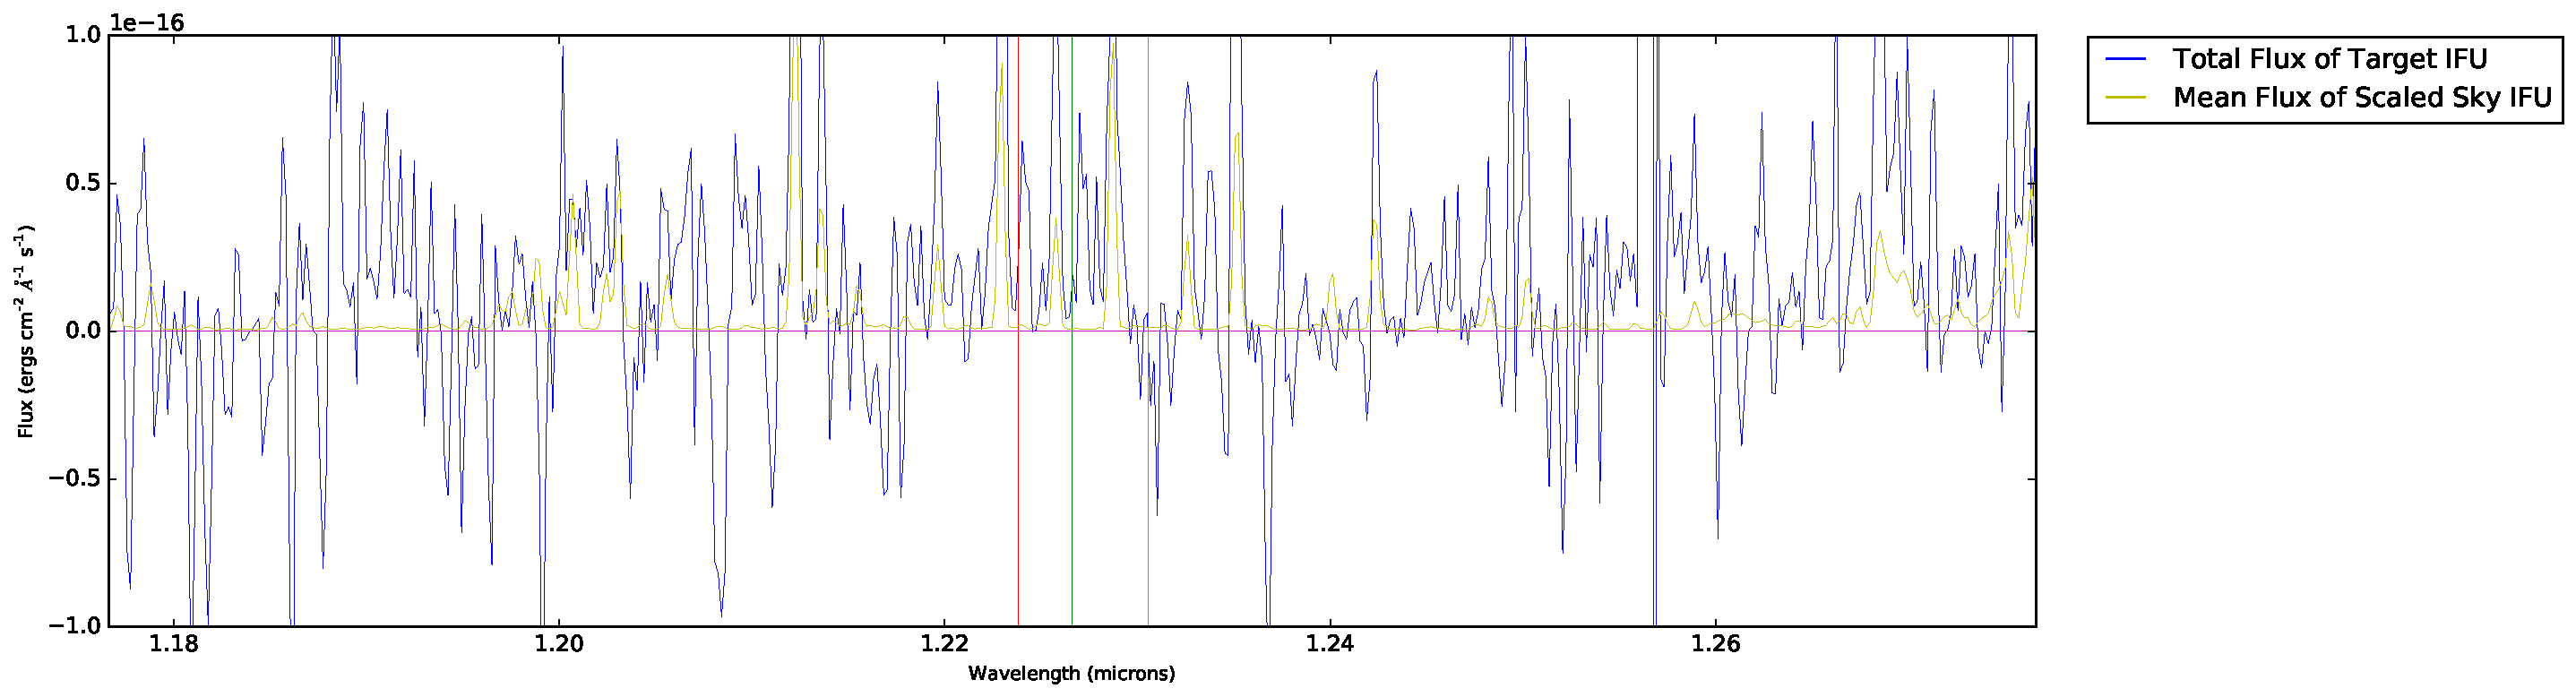
\includegraphics[scale=0.4]{figures/CL0034-YJ-OB-1_2014-07-11Tfirst_exposure_Target_5.pdf}
\end{figure}
%/home/rburnet/S16work/formal_documentation/figures/CL0034-YJ-OB-1_2014-07-11Tfirst_exposure_Target_5.pdf

We then collapsed the cubes between the two NII lines around H$\alpha$ to see if we could pick out a source to define an aperture around to extract the spectrum of. They all seemed to show a region of bright pixels that could be a galaxy to define an aperture around. I defined an aperture to extract total flux averaged from each exposure (all 5 from both OB1 and OB2) for each target and plotted them (see \\$\sim$/S16work/manual$\_$sky$\_$subtraction$\_$scripts/target$\_$sky$\_$fraction$\_$of$\_$IFU$\_$specific$\_$targets$\_$specific$\_$regions$\_$exposures$\_$averaged.py). See figure below of CL0034 target 5 (see \\$\sim$/S16work/figures/laptop/target$\_$sky$\_$fraction$\_$of$\_$object/sky$\_$subtracted$\_$spectrum$\_$of$\_$IFUs/specific$\_$targets$\_$specific$\_$regions$\_$\\exposures$\_$averaged/ for the rest of the images).\\

\begin{figure}[h!]
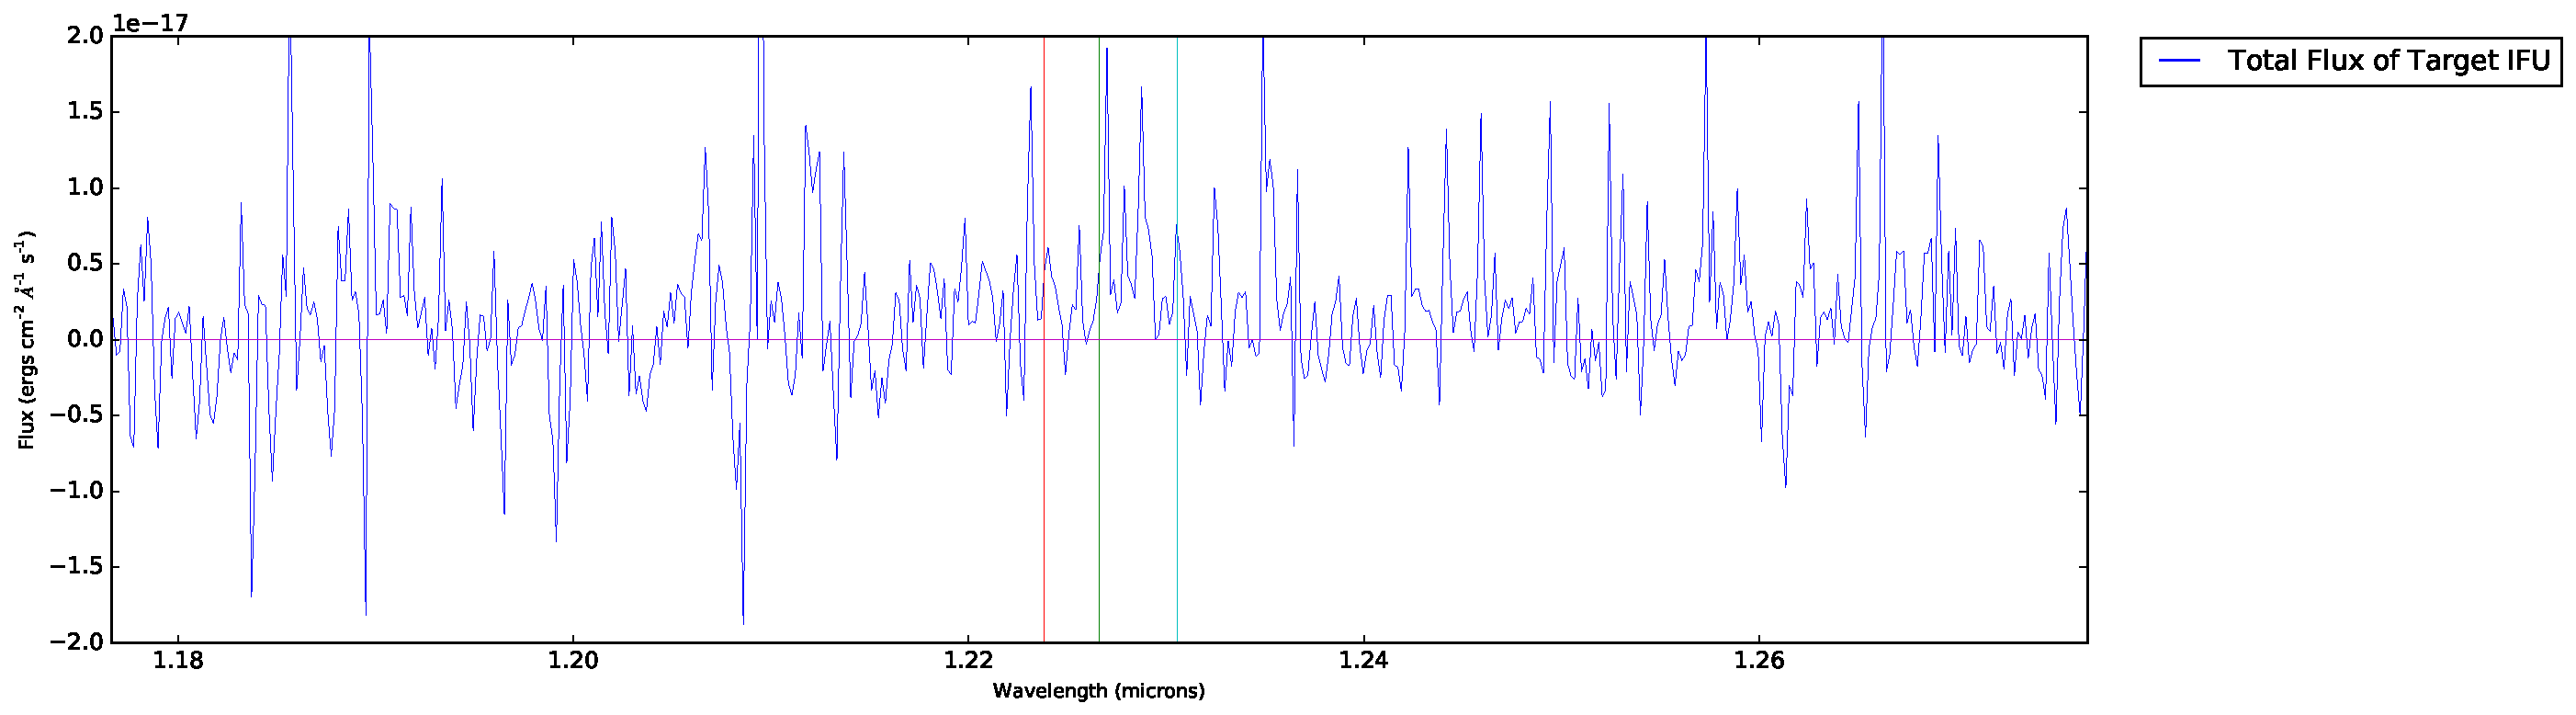
\includegraphics[scale=0.4]{figures/CL0034-YJ_Target_5_specific_region.pdf}
\end{figure}
%/home/rburnet/S16work/formal_documentation/figures/CL0034-YJ_Target_5_specific_region.pdf

Unfortunately, still no H$\alpha$ detection. Our next step was to look into the reduced IZ data cubes (all 5 from both OB1 and OB2) and extract the spectrum to find OII and H$\beta$, but once again to no avail (see \\$\sim$/S16work/manual$\_$sky$\_$subtraction$\_$scripts/target$\_$sky$\_$fraction$\_$of$\_$IFU$\_$specific$\_$targets$\_$specific$\_$regions$\_$exposures$\_$averaged$\_$IZ.py). See figure below of CL0034 target 5 (see \\$\sim$/S16work/figures/laptop/target$\_$sky$\_$fraction$\_$of$\_$object/sky$\_$subtracted$\_$spectrum$\_$of$\_$IFUs/specific$\_$targets$\_$specific$\_$regions$\_$\\exposures$\_$averaged$\_$IZ/ for the rest of the images).\\

\begin{figure}[h!]
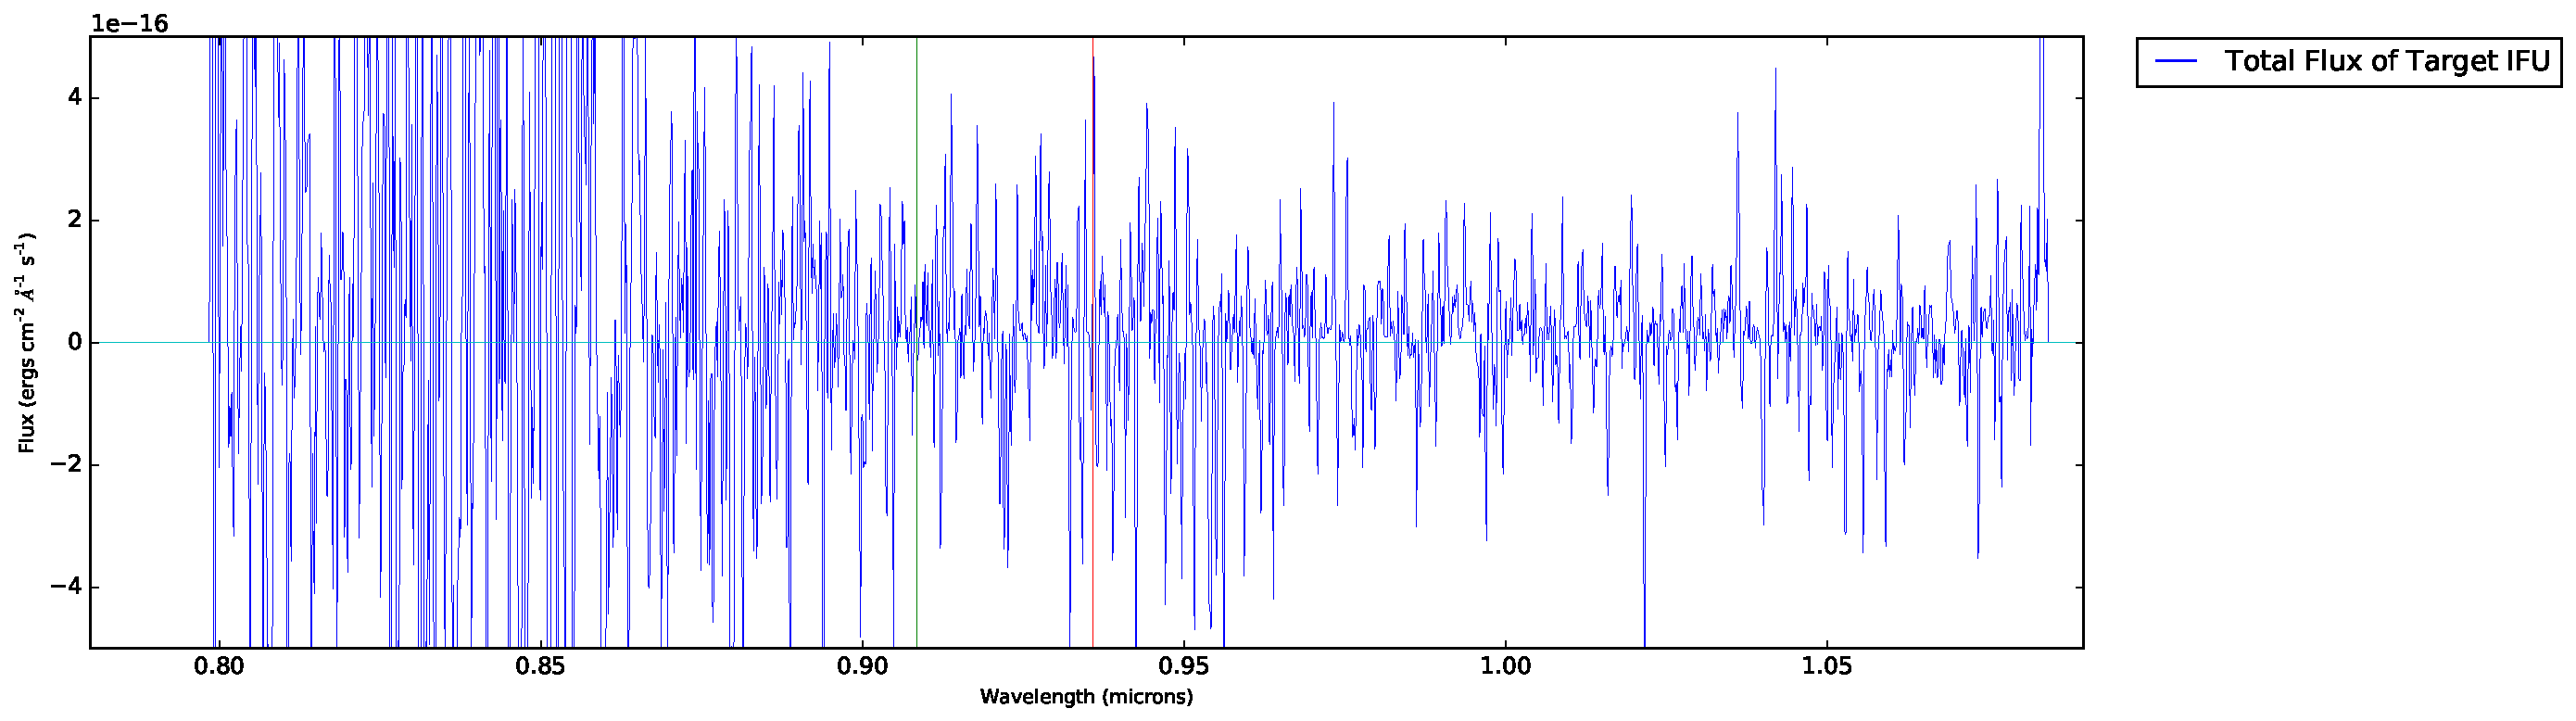
\includegraphics[scale=0.4]{figures/CL0034-IZ_Target_5_specific_region.pdf}
\end{figure}
%/home/rburnet/S16work/formal_documentation/figures/CL0034-IZ_Target_5_specific_region.pdf

We expected to see some OII and H$\beta$, but just like with H$\alpha$, we found nothing.

\subsection{June 8: Combining cubes, new manual sky subtraction}
We came up with a slightly different method of sky subtraction than the one detailed in the last section. Instead of scaling the mean sky flux to the target's perimeter mean flux like:\\
f = $\frac{\text{T}_{\lambda}\text{(perimeter)}}{\text{S}_{\lambda}\text{(sky)}}$\\
we used the sky arms total flux from the science frame (S$_{sci}$) to scale it's corresponding sky arm total flux from the sky frame (S$_{sky}$), and used that scale factor to scale the sky arm corresponding to the target arm like:\\
f = $\frac{\text{S}_{sci}}{\text{S}_{sky}}$\\
we did it this way, using the sky arms from the science frames, because some of the sources extend beyond the FOV of the arms, so using the perimeter of the data cubes as sky would not be representative of the true sky for those objects (see figure below of HST image of CL0036 target 26). By using the sky arm from the target frame to scale the sky arm from the sky frame to the target arm flux, we guarantee we are scaling the skies properly (see $\sim$/S16work/manual$\_$sky$\_$subtraction$\_$scripts/using$\_$sky$\_$arms.py\\

\begin{figure}[h!]

\includegraphics[scale=0.4]{figures/CL0036-Target_26.png}
\end{figure}
%/home/rburnet/S16work/formal_documentation/figures/CL0036-Target_26.png

This method of sky subtraction was applied to the combined cubes of all 5 exposures for every target in the YJ-band and IZ-band separately. I combined the cubes using the esorex pipeline ``kmos$\_$combine" (see document \cite{KMOS pipeline manual}, specifically recipe kmos$\_$combine, for details).\\

To combine cubes, I retrieve the files from the pipeline final products called\\ CL003[4|6]-[Y|I][J|Z]-OB-[1|2]$\_$SCI$\_$RECONSTRUCTED$\_$KMOS*, put the two OBs together in one directory, created an sof file called ``combine.sof" that lists each of the files to be combined followed by the designation ``CUBE$\_$OBJECT", then ran in terminal:\\

esorex kmos$\_$combine -method='header' combine.sof\\

This combined the cubes listed in combine.sof by target name and outputted each of the combined targets and their exposure masks in the same directory.\\

I then applied the above manual sky subtraction method to these combined cubes. However, a problem arose in that the target cube total flux over the whole spectrum seemed to be negative for a few data cubes, resulting in us not being able to calculate magnitudes for these cubes (to be used in the diagnostic report, more on that later). This was the case for CL0034 target 11, which is supposed to be the brightest target in that cluster.

\subsection{June 15: Pipeline sky subtraction with local sky subtraction, diagnostic report}
Due to the total flux for some cubes over the whole spectrum being negative, we first attempted to reduce the data without any calibration to see if at any step in the calibration the reduced data cubes result in negative flux, but even without calibration the reduced data cubes (especially target 11) still had negative total flux. So we instead ran the pipeline with sky subtraction and sky tweak, combined the reduced pipeline data cubes for each observation block (OB1 and OB2), and then subtracted the flux of the target to it's local sky to ensure the target flux was positive. By this, I mean we defined an aperture around a bright central region of each of the pipeline sky subtracted data cubes and defined the local sky to be all the spaxels outside of this aperture. We median combine the local sky flux and subtract this sky flux from each of the spaxels in the target cube for each wavelength slice. This ensures that the total local sky flux after sky subtraction is 0, and the total flux within the aperture is positive. We then plotted the spectrum for both the IZ and YJ bands for each target cube and it's corresponding sky cube (see $\sim$/S16work/diagnostic$\_$of$\_$objects/local$\_$sky$\_$subtraction/local$\_$sky$\_$subtraction$\_$sky$\_$arm$\_$sky$\_$frame$\_$as$\_$sky$\_$flux.py). See the below figure of CL0034 target 2 spectrum plot in the YJ-band as an example (see \\/home/rburnet/S16work/diagnostic$\_$of$\_$objects/local$\_$sky$\_$subtraction/figures/ for more plots)\\

\begin{figure}[h!]
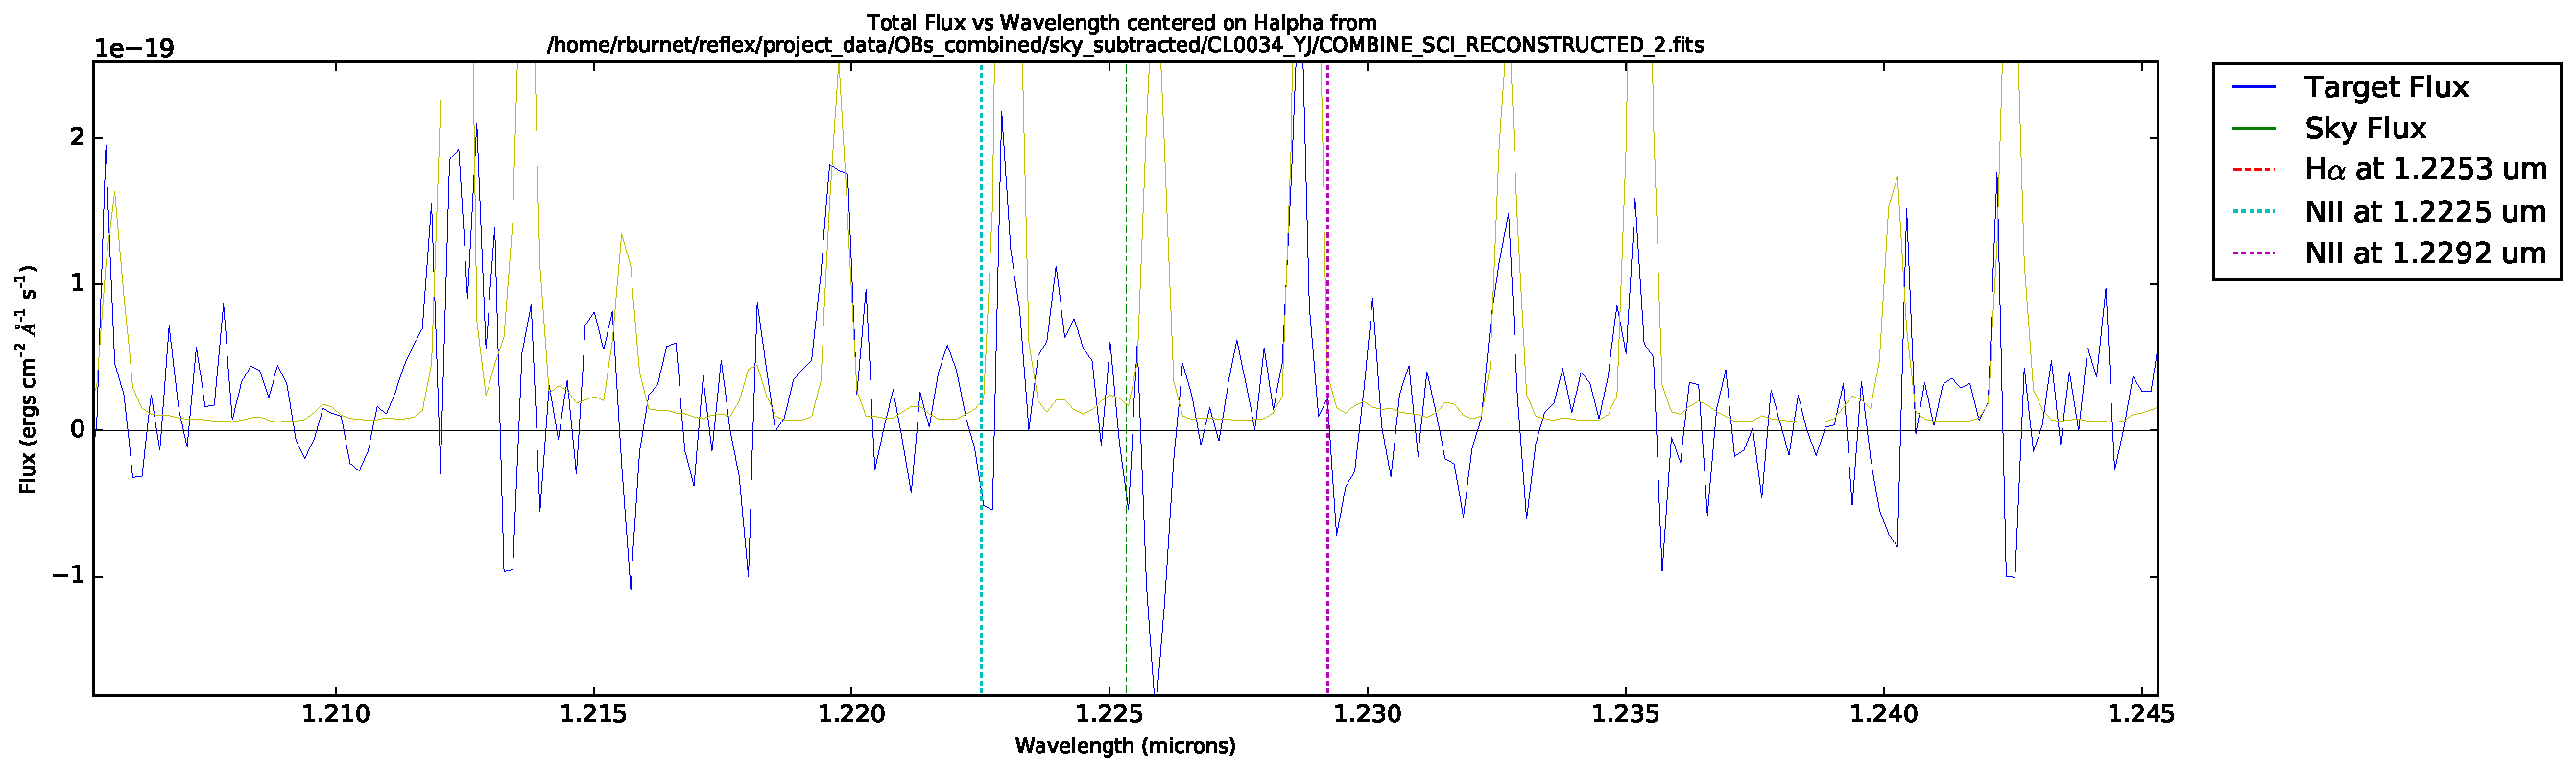
\includegraphics[scale=0.4]{figures/COMBINE_SCI_RECONSTRUCTED_2_Halpha.pdf}
\end{figure}
%/home/rburnet/S16work/formal_documentation/figures/COMBINE_SCI_RECONSTRUCTED_2_Halpha.pdf

With this, it was time to create the diagnostic report.\\

The diagnostic report is the last thing I created and did for the KMOS data. It was essentially a compilation of all the important information for each reduced data cube to be sent to Sean for him to look at and to have on hand in case in the future we'd want to look back on the KMOS data. The diagnostic report contains the HST images of all the targets at that we could find with the same pointing, orientation, and FOV as the data cubes, the collapsed images of the combined OBs of the targets for both the YJ and IZ bands, calculated YJ and IZ magnitudes, calculated expected H$\alpha$ flux from SFR(OII) values as detailed in Sean's catalogue, and the relevant spectra.\\

The HST images were provided to me by Micheal. I opened them in DS9, oriented them to the KMOS data cubes, and took a snapshot of the FOV of the data cubes by creating and importing a square region from the data cubes that covered the whole area of the data cubes into the HST images. The collapsed images were created using the esorex kmos recipe ``kmo$\_$make$\_$image" (see kmo$\_$make$\_$image recipe in document \cite{KMOS pipeline manual}). The YJ and IZ magnitudes were calculated using the relationship M = -2.5$\times$log($\frac{Flux}{0.1 \times F_0}$) where $Flux$ is the median of the total flux within the aperture of the target cubes over all wavelength slices, $F_0$ is the zero point flux of the filter/band, and 0.1 is the unit conversion between ergs/s/cm$^2$ and W/m$^2$. H$\alpha$ flux is calculated using the K98 SFR(H$\alpha$) relation from article \cite{K98} where I go from SFR(OII) = SFR(H$\alpha$) -$>$ L(H$\alpha$) -$>$ Flux(H$\alpha$). To go from L(H$\alpha$) -$>$ Flux(H$\alpha$) I used the flux-luminosity relation with the distance being the luminosity distance calculated from the target's redshift. The astropy.cosmology module for python can calculate the luminosity distance for you. The spectra are simply the total flux vs wavelength of the target cubes and sky cubes overlaid on top of one another using the local sky subtraction method detailed above. The apertures defined are shown in the collapsed images as green outlines.\\

To see the diagnostic report, go to $\sim$/S16work/diagnostic$\_$of$\_$objects/local$\_$sky$\_$subtraction/new$\_$report/ . An older, deprecated diagnostic report is in $\sim$/S16work/diagnostic$\_$of$\_$objects/report/ .\\

After this, there was no where else we could go until we heard back from Sean. So we moved on to a new project involving SAMI data and ALFALFA survey data on July 4.

\end{document}